\resetfigpath{Chap4}

%%%{INTRODUCTION to this CHAPTER}%%%

In Chapter ~\ref{chap:DriverModel}, a model providing a probabilistic way to evaluate the possible behaviors of other traffic participants was proposed. The concept of the fact that TFA distributions are different among people was also elaborated and formulated in Eqn.~\ref{eq:TFA_est}. Then, the average parameter of participants were found and used to estimate the POY in the experiment at the simulated crossroad. In this chapter, the characteristic parameters of drivers will be attempted to identify.


%%%%%%%%%%%%%%%%%%%%%%%%%%%%%%%%%%%%%%%%%%%%%%%%%%%%%%%%%%%%%%%%%%%%%%%%
%%%%%%%%%%               SECTION SECTION SECTION               %%%%%%%%%
%%%%%%%%%%%%%%%%%%%%%%%%%%%%%%%%%%%%%%%%%%%%%%%%%%%%%%%%%%%%%%%%%%%%%%%%
\section{Characteristic Parameters}
\label{sec:characterParam}

The way people drive is different from person to person, some are aggressive, while others are more conservative. This also applies to the decision on braking moment. In Section ~\ref{sec:TFADistribution}, the mean value of TFA distribution of drivers is formulated in Eqn.~\ref{eq:TFA_est}, where three parameters including $R_{min}$ and $a_{dec}$ are introduced. The $R_{min}$, standing for the minimum distance left when the vehicle is fully stopped, being a parameter known as a function of velocity of the vehicle, is also changing with different characters. To put it another way, two different driver driving two identical vehicles under same speed would have different mean distance left before the vehicle and the obstacle when the vehicle stops moving. This is a rather instinctive results since a more aggressive people tend to brake as late as possible which contributes to the smaller $R_{min}$. Similarly, drivers who make traffic offense are having higher $a_{dec}$ than those more conservative.

What can be learned from Eqn.~\ref{eq:TFA_est} is that, each of these parameters can put effect on the value of ${TTA}_{est}$, in other words, they decide the value of ${TTA}_{est}$ and the results of POY. In Fig.~\ref{fig:trial003params} and Fig.~\ref{fig:trial077params}, the POY using the average parameters and the driver's parameters are compared. As we can see in these cases, the POYs of the vehicle (car\_0 in Fig.~\ref{fig:trial003}) are higher using the characteristic parameters belonging to the driver. 



\begin{figure}[htbp!]
\begin{center}
\makebox[0pt]{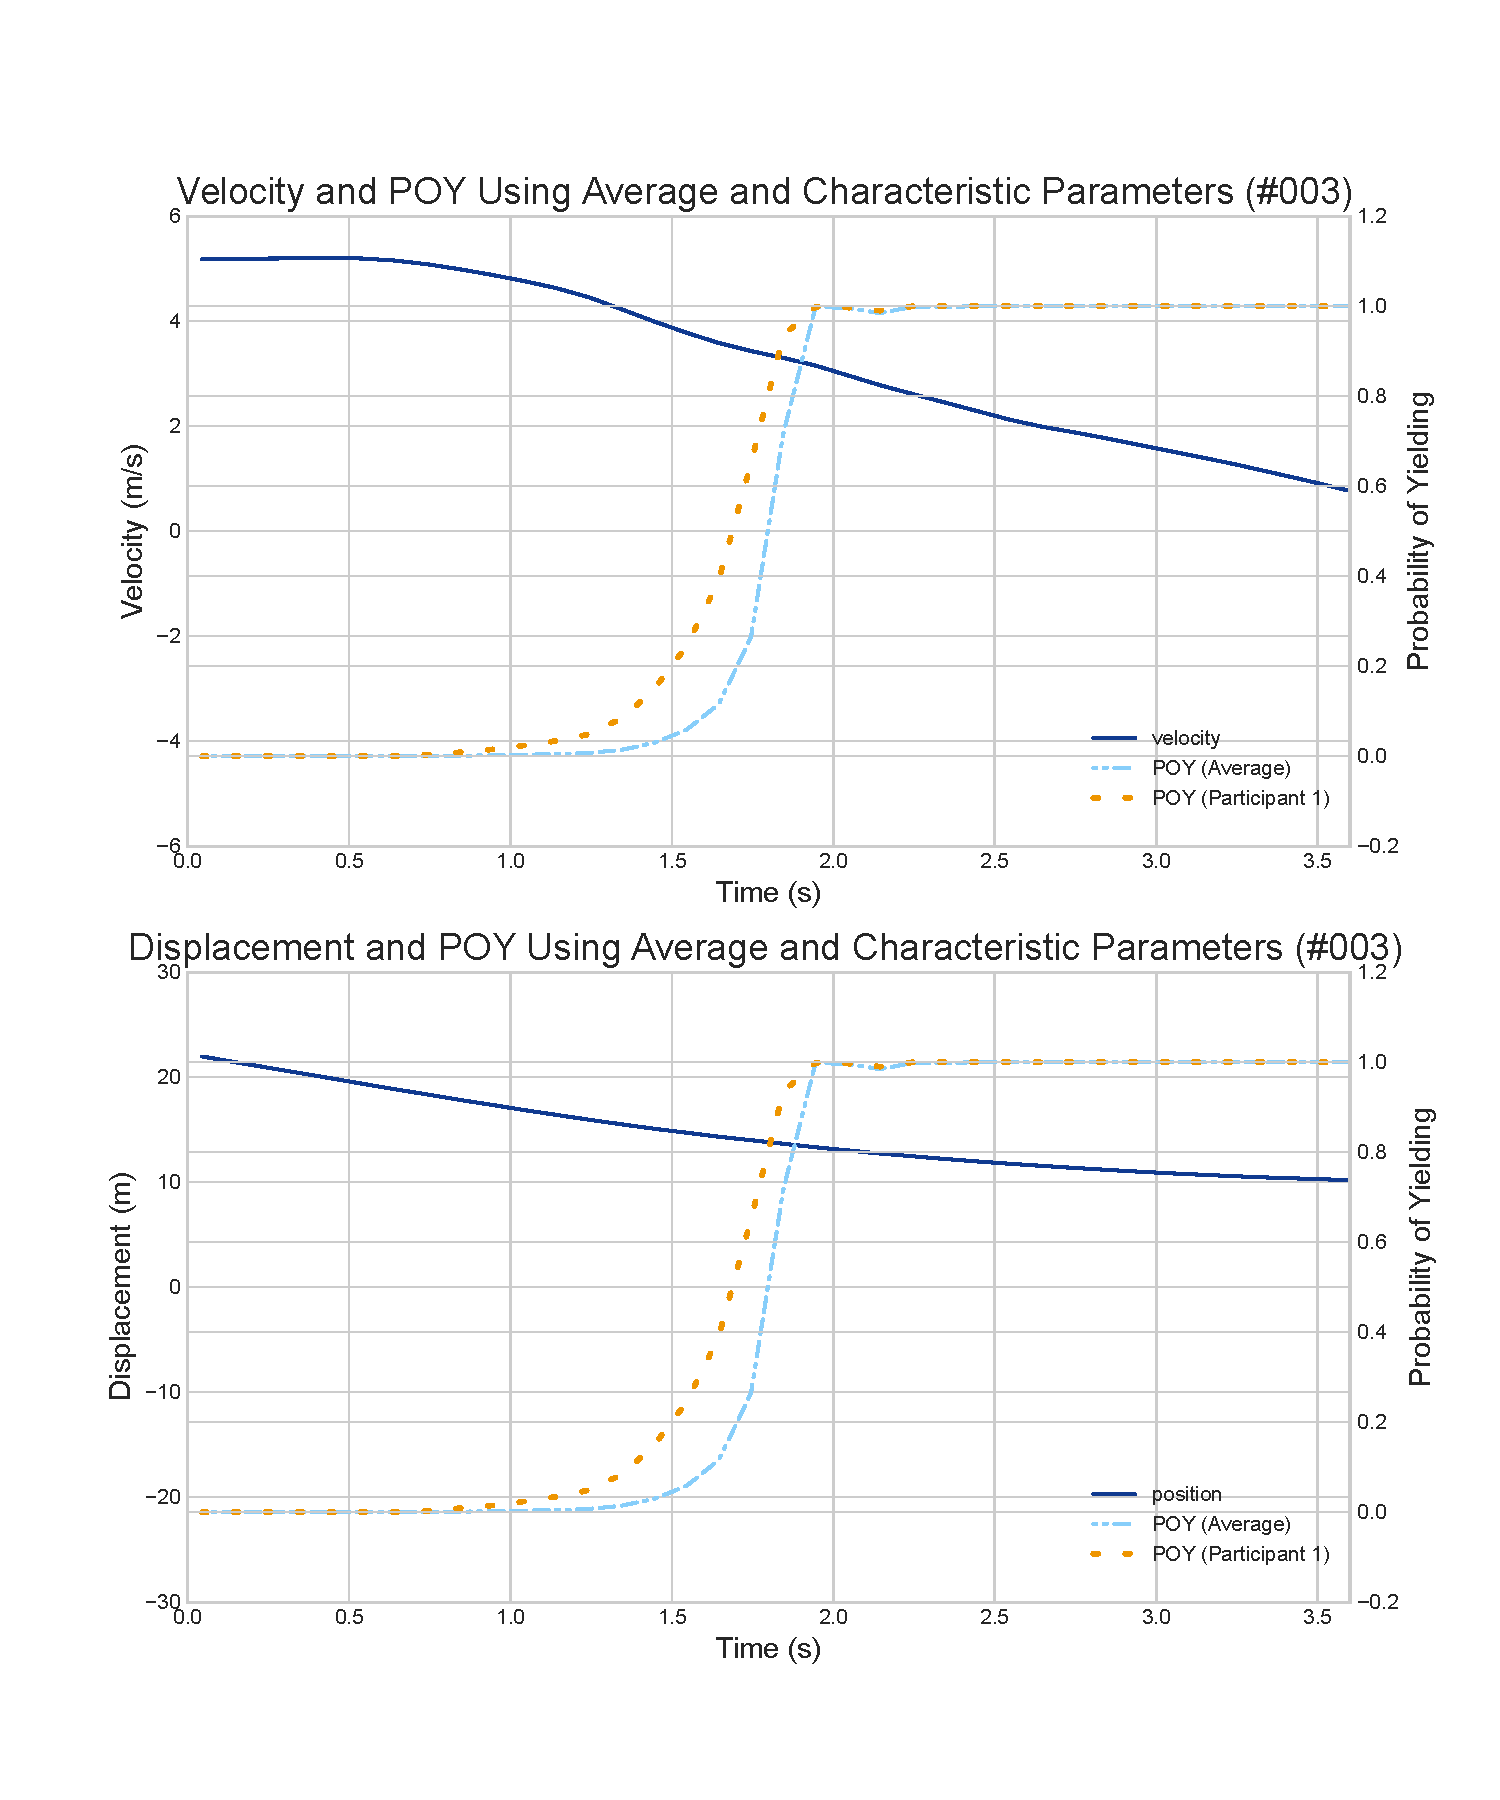
\includegraphics[width=0.65\paperwidth]{compare_trial_003.pdf}}
\end{center}
\caption{Trial \#003 with POY using average parameters and parameters of Participant 1.}
\label{fig:trial003params} 
\end{figure}

\begin{figure}[htbp!]
\begin{center}
\makebox[0pt]{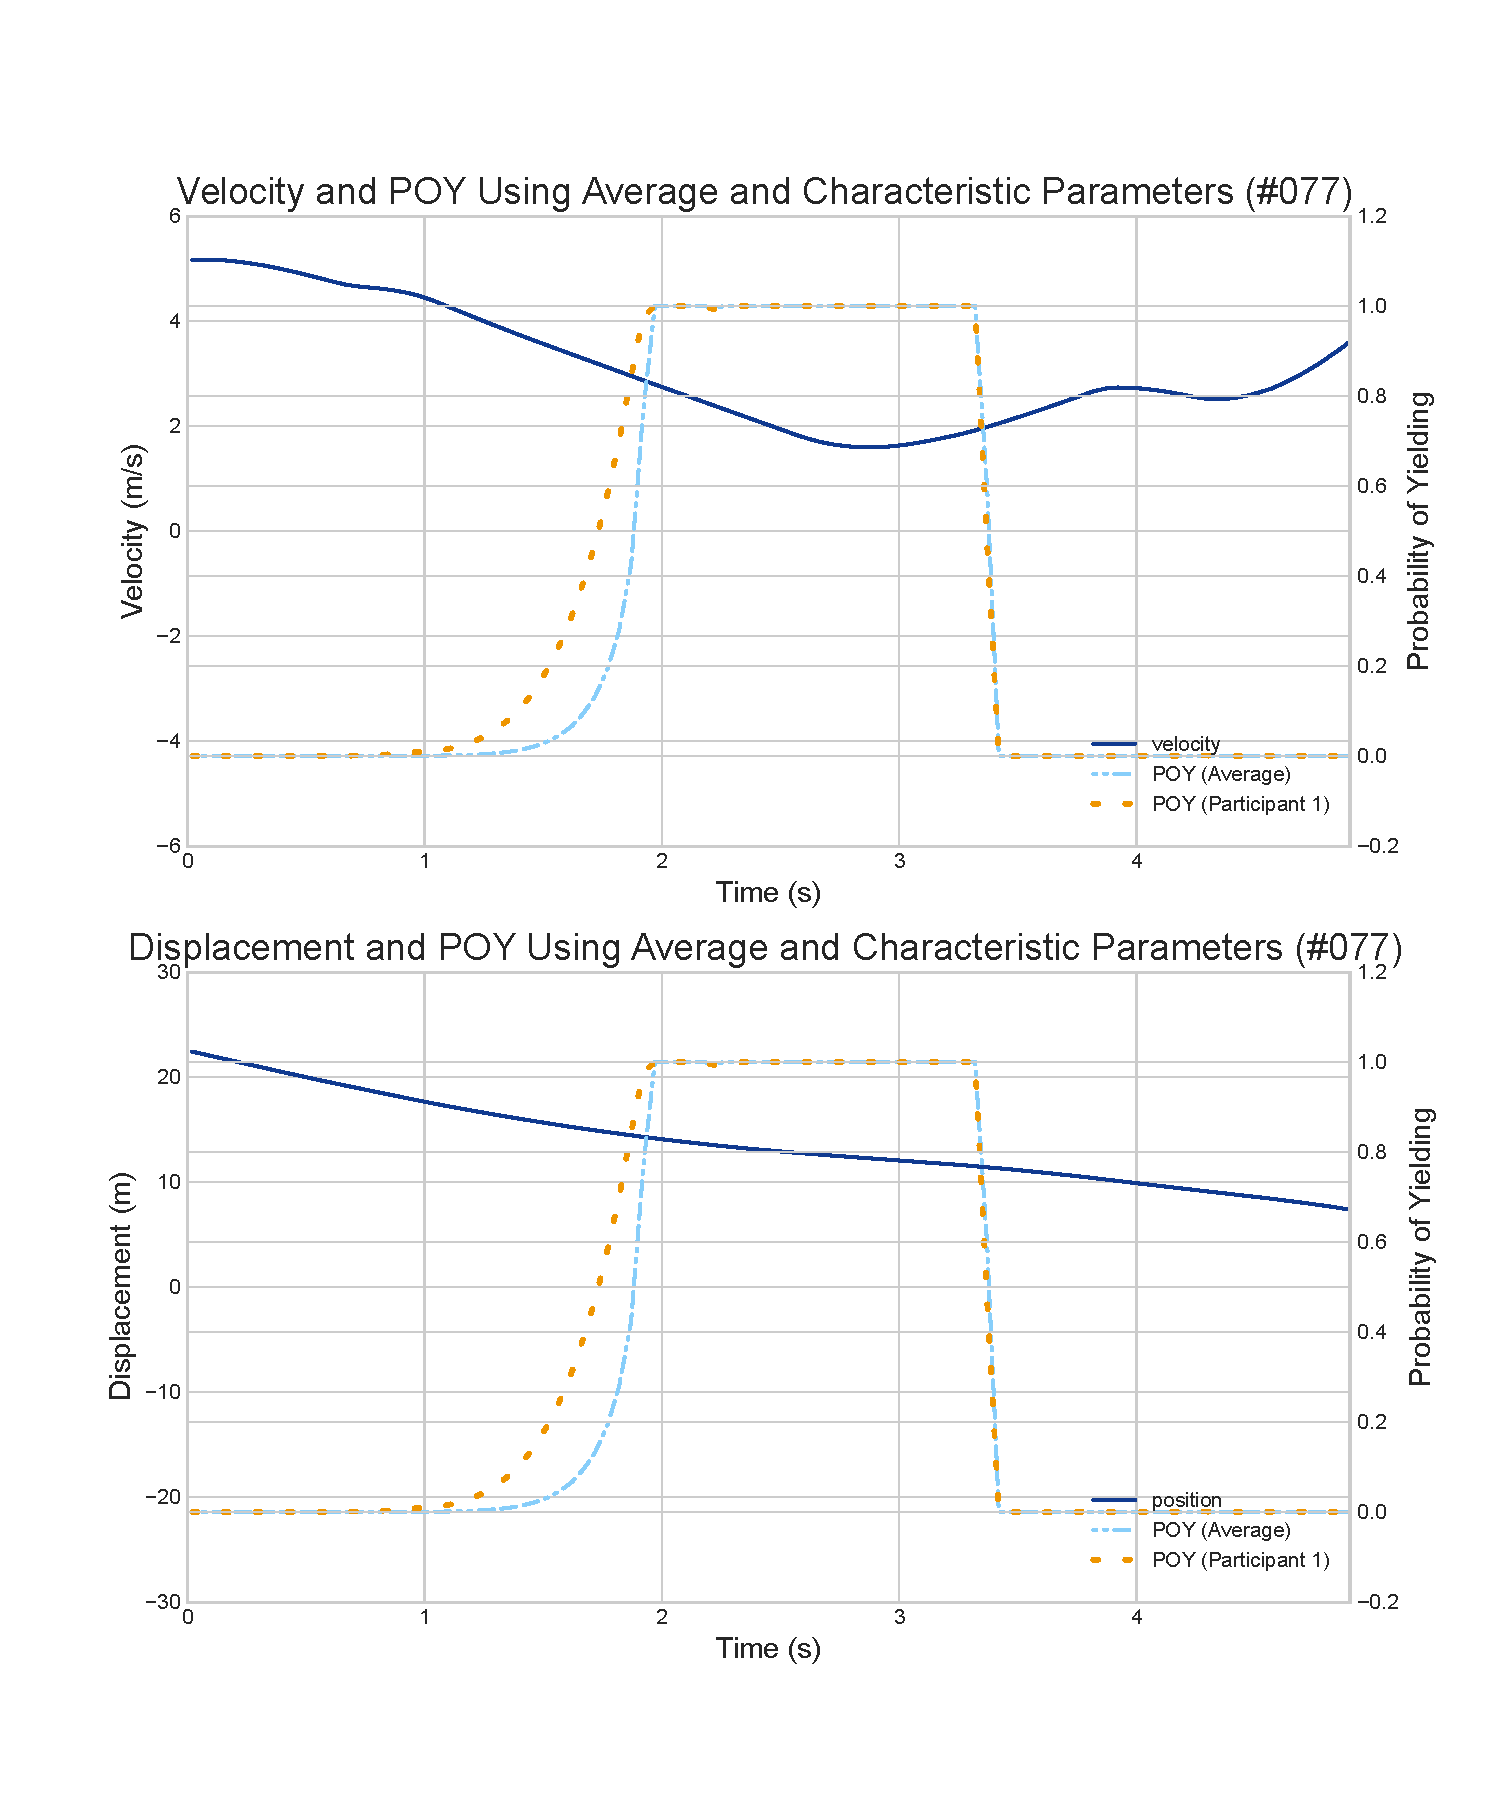
\includegraphics[width=0.65\paperwidth]{compare_trial_077.pdf}}
\end{center}
\caption{Trial \#077 with POY using average parameters and parameters of Participant 1.}
\label{fig:trial077params} 
\end{figure}


This phenomenon is owing to the closer estimation of the TFA distribution. Bringing a set of average parameters into Eqn.~\ref{eq:TFA_est} will only give an rough whereabouts of the TFA of the driver at the moment (considering velocity, displacement to the node and so on). Using the specific characteristic parameters, on the other hand, could effectively narrow down the TFA of the driver to within the consequential TFA distribution. Still, chances are that the estimated TFA distribution using the characteristic parameter might be different from the real TFA under the circumstance, given that both of them are distributions. However, given a large enough database, the average POY acquired using characteristic parameters should be higher than that using average parameter.


\begin{figure}[htbp!]
\begin{center}
\makebox[0pt]{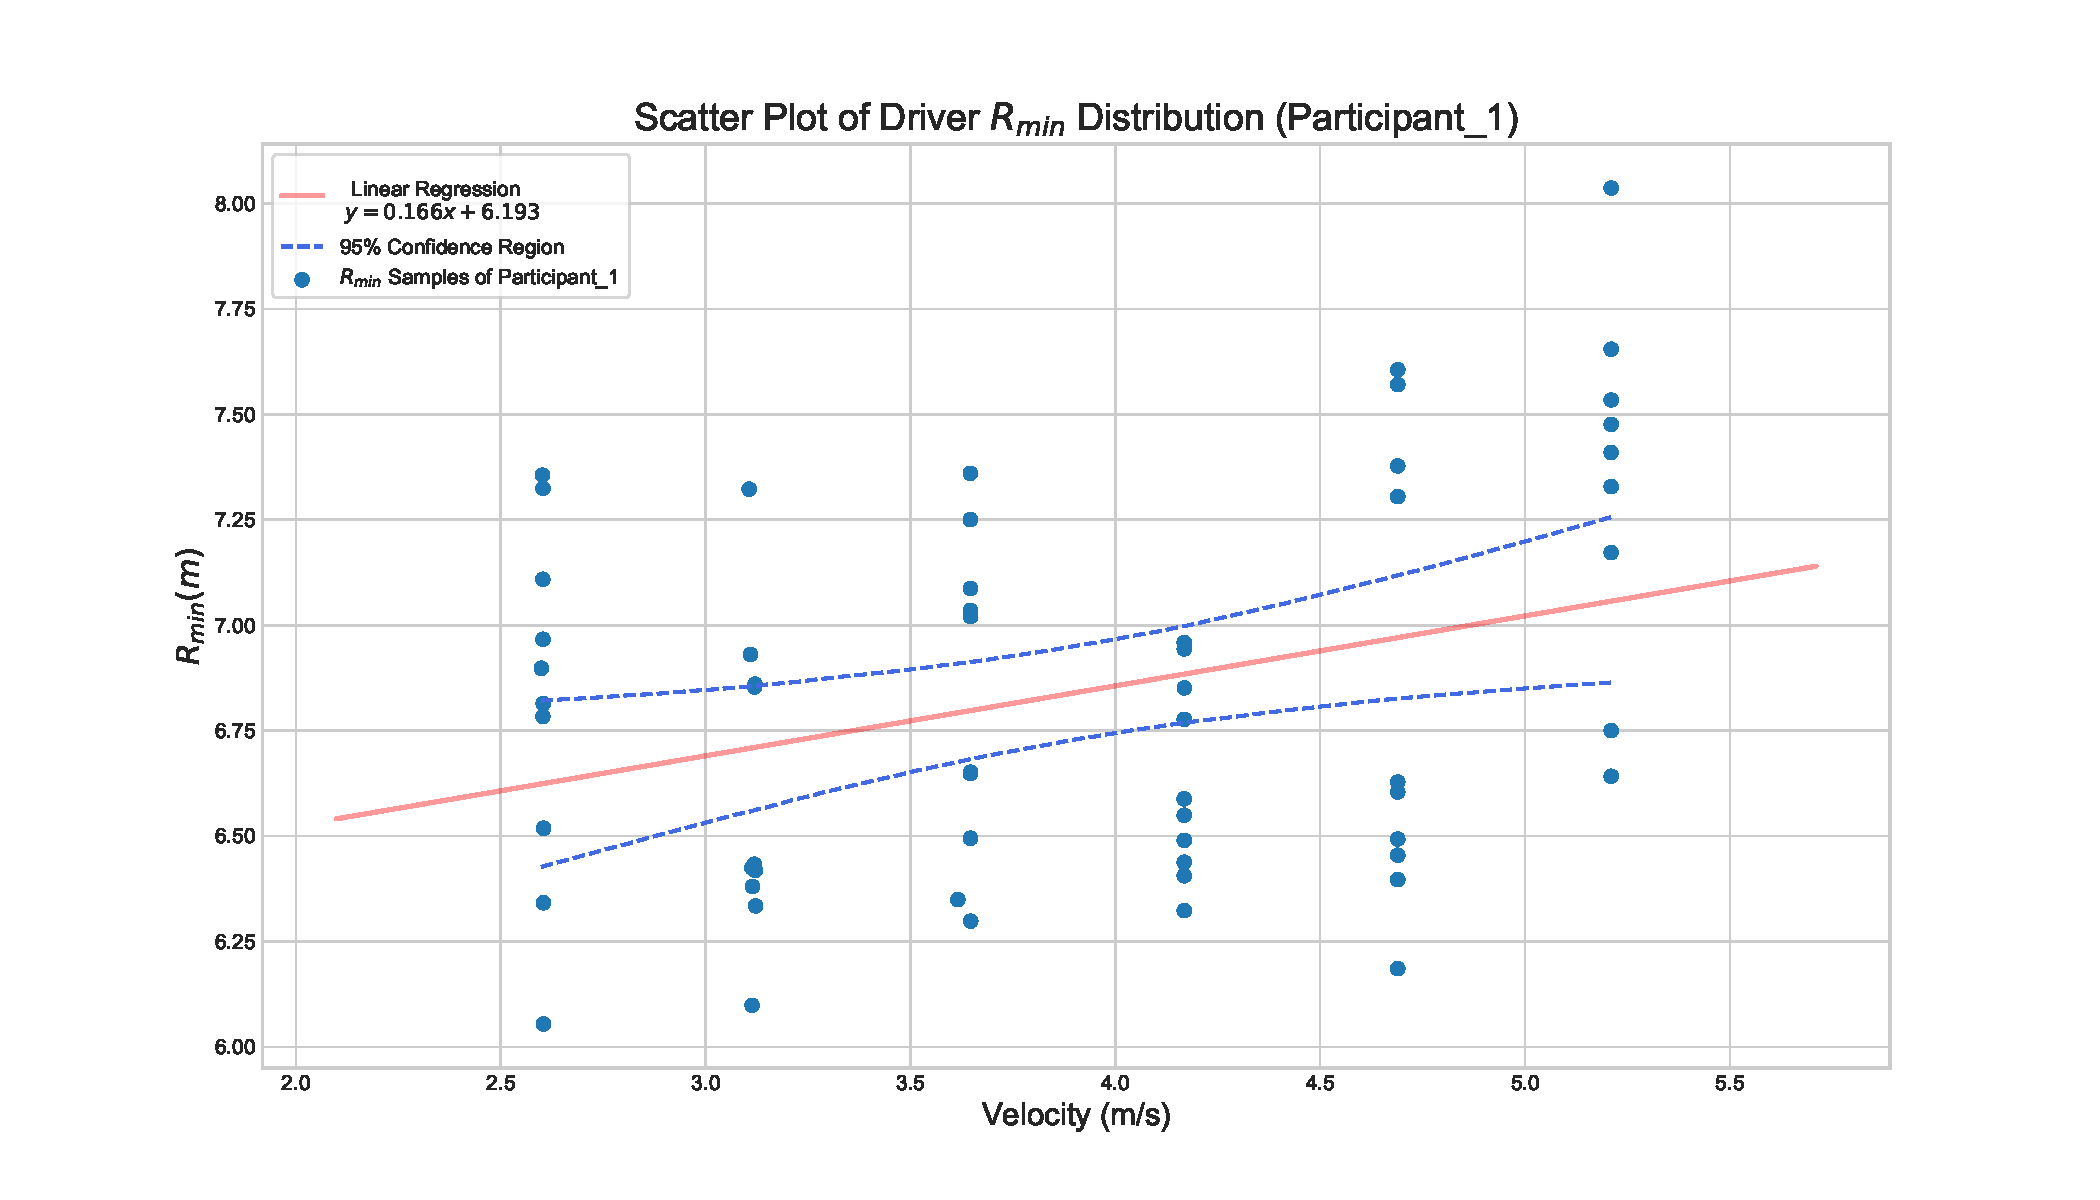
\includegraphics[width=0.7\paperwidth]{/Participant_1_R_MIN_polyfit.pdf}}
\end{center}
\caption{The $R_{min}$ scatter plot of Participant 1 under various velocities.}
\label{fig:Par1RMINDifSpeed} 
\end{figure}

\begin{figure}[htbp!]
\begin{center}
\makebox[0pt]{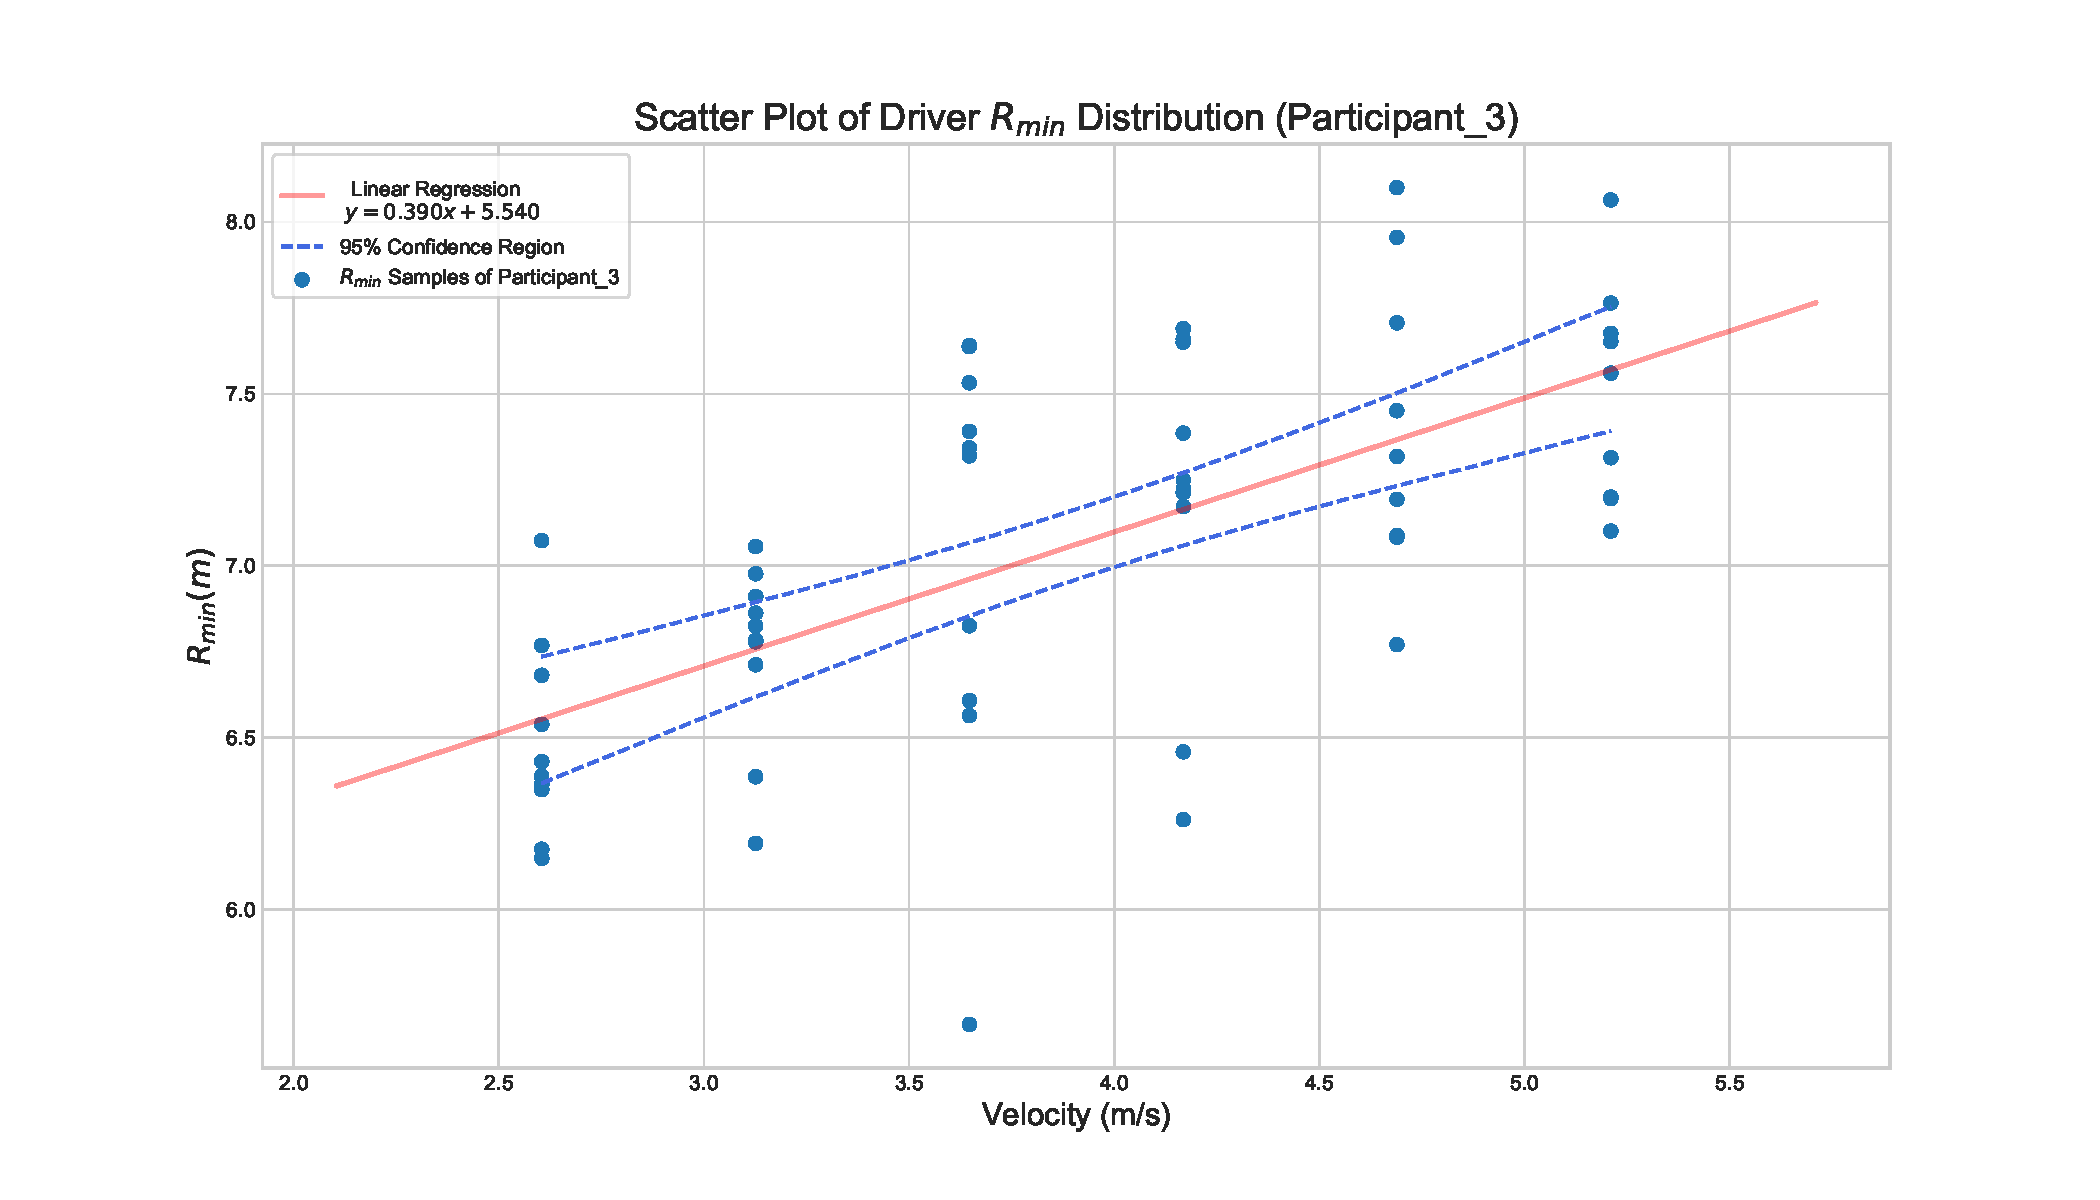
\includegraphics[width=0.7\paperwidth]{/Participant_3_R_MIN_polyfit.pdf}}
\end{center}
\caption{The $R_{min}$ scatter plot of Participant 3 under various velocities.}
\label{fig:Par3RMINDifSpeed} 
\end{figure}

\begin{figure}[htbp!]
\begin{center}
\makebox[0pt]{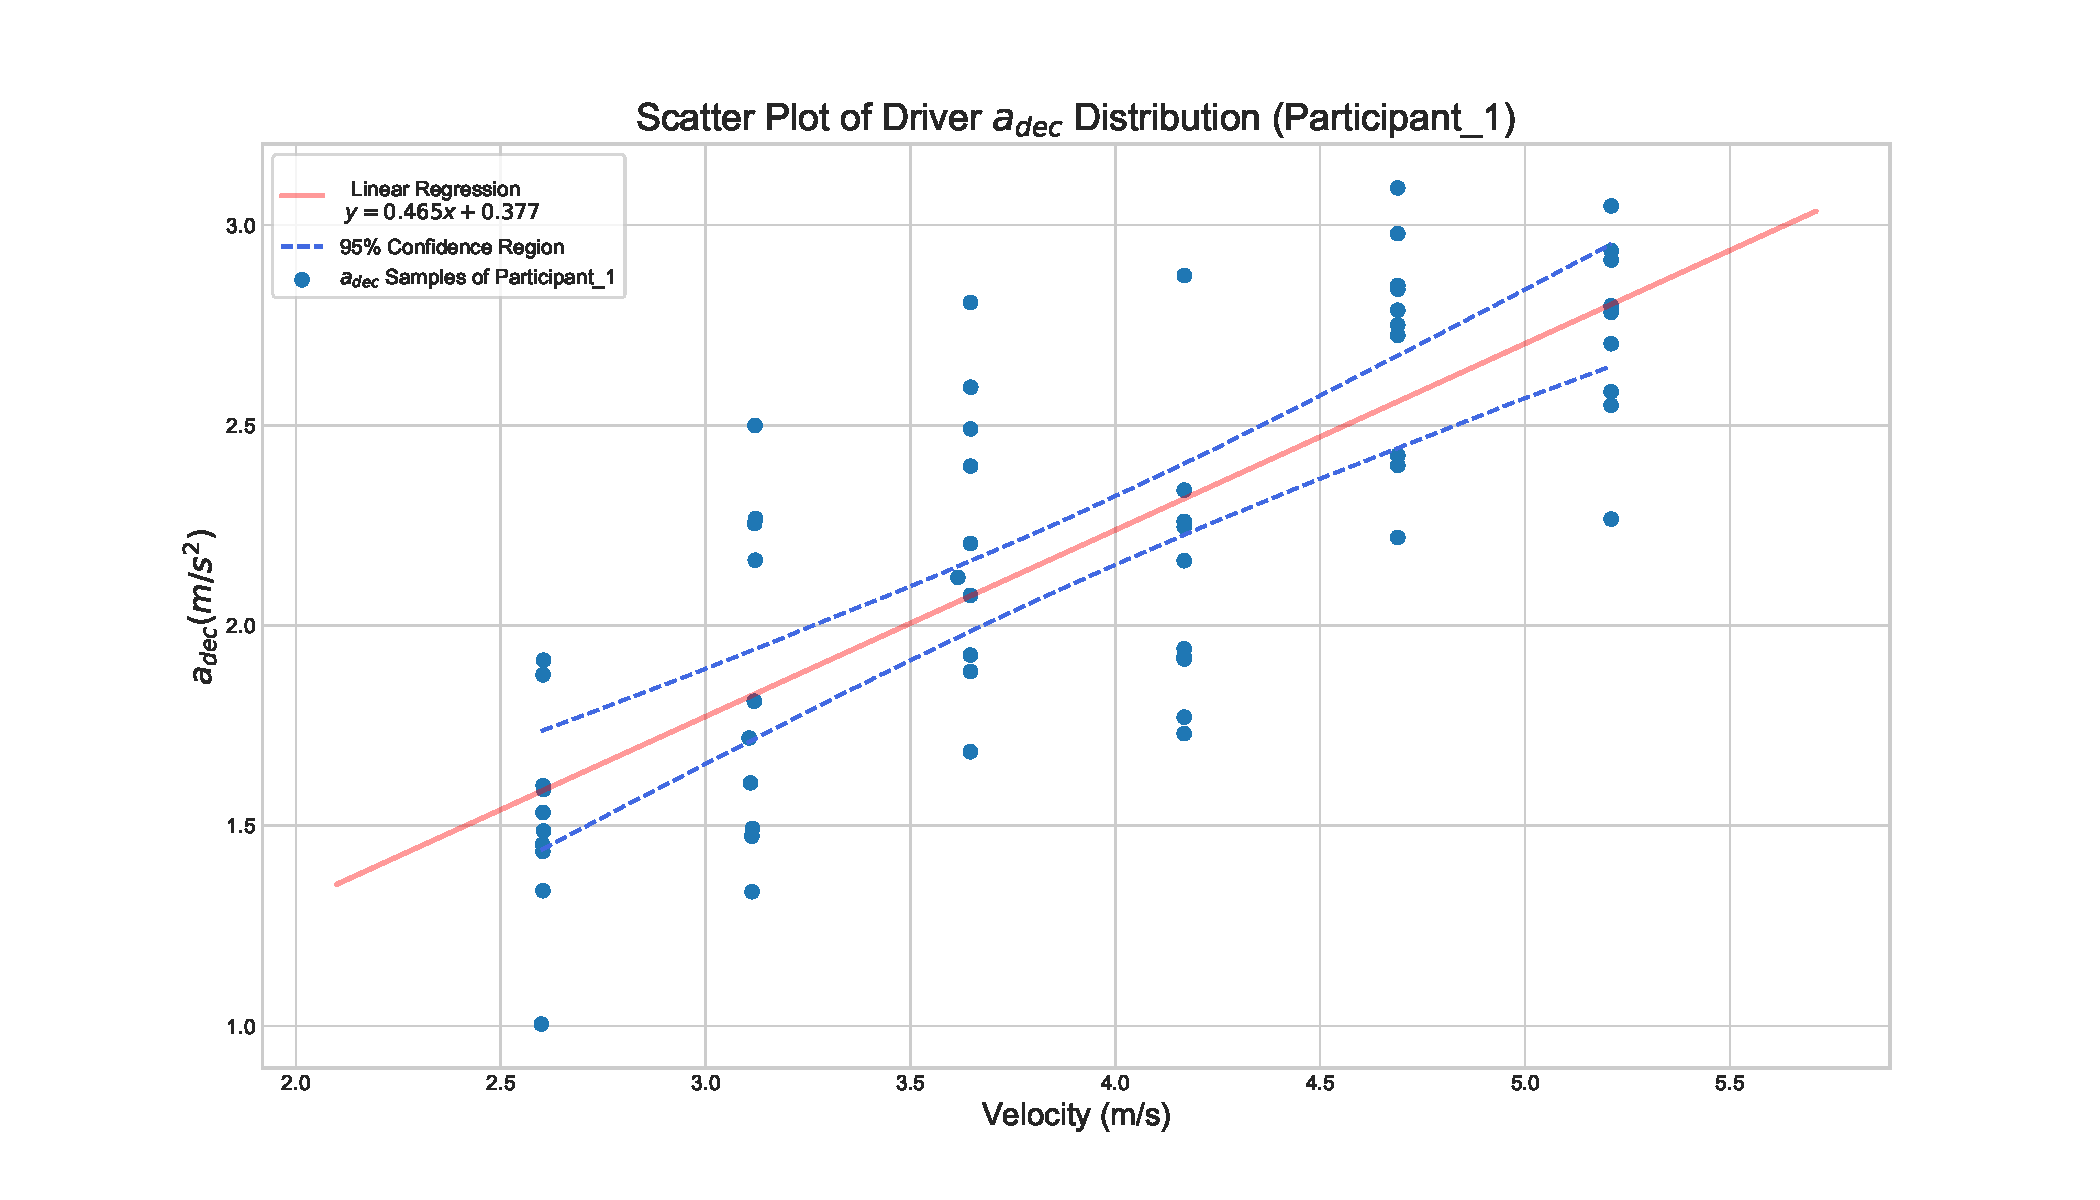
\includegraphics[width=0.7\paperwidth]{/Participant_1_A_DEC_polyfit.pdf}}
\end{center}
\caption{The $a_{dec}$ scatter plot of Participant 1 under various velocities.}
\label{fig:Par1ADECDifSpeed} 
\end{figure}

\begin{figure}[htbp!]
\begin{center}
\makebox[0pt]{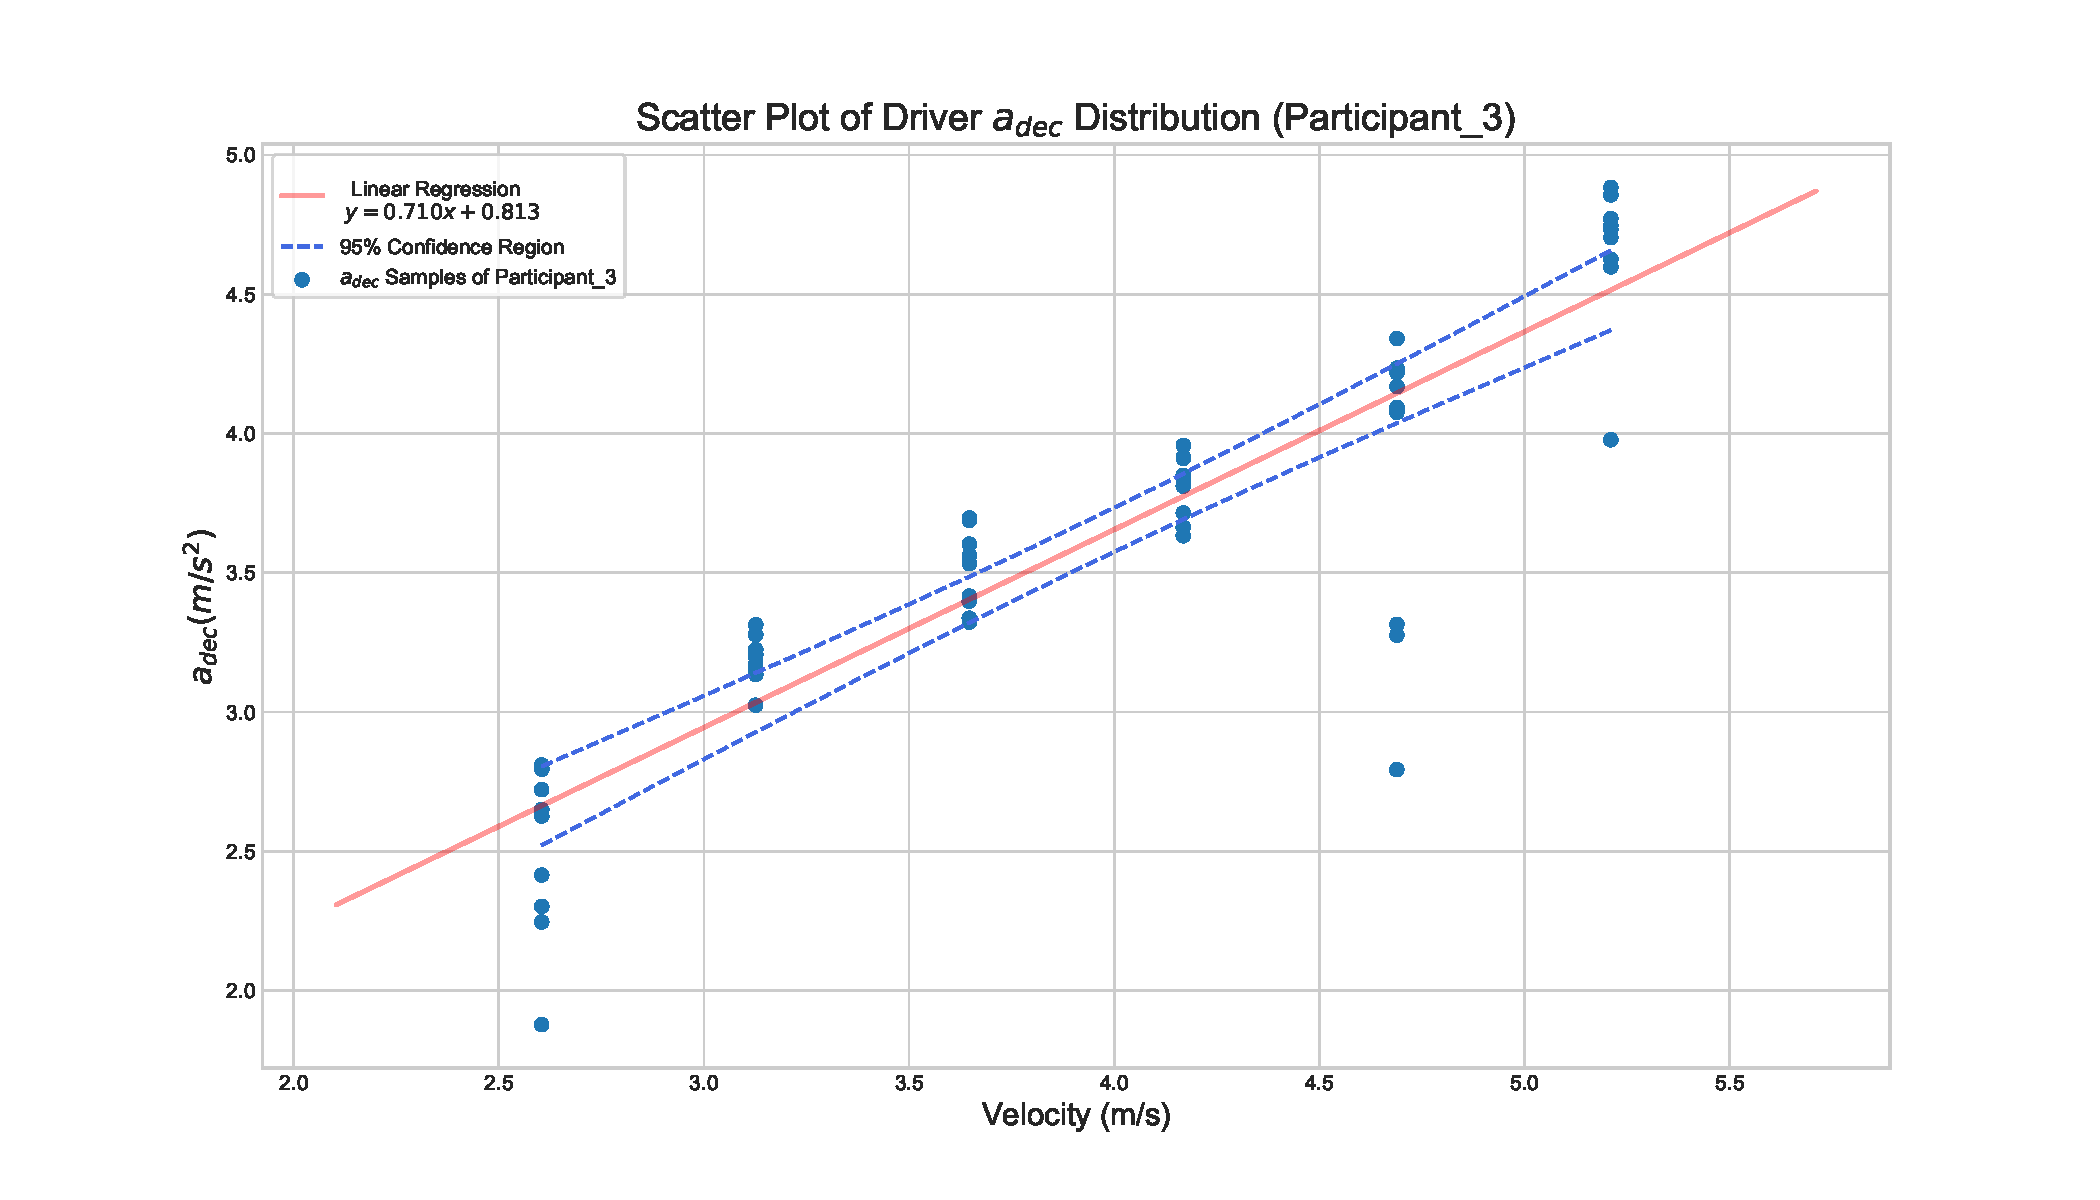
\includegraphics[width=0.7\paperwidth]{/Participant_3_A_DEC_polyfit.pdf}}
\end{center}
\caption{The $a_{dec}$ scatter plot of Participant 3 under various velocities.}
\label{fig:Par3ADECDifSpeed} 
\end{figure}

To identified the corresponding characteristic parameters of participants, experiments same as the one used in Chapter ~\ref{chap:DriverModel} are conducted for each participants. Here, experimental results and characteristic parameters of Participant 1 and 3 are shown in Fig~.\ref{fig:Par1RMINDifSpeed}, Fig~.\ref{fig:Par1ADECDifSpeed}, Fig~.\ref{fig:Par3RMINDifSpeed} and Fig~.\ref{fig:Par1ADECDifSpeed}. 

Similar to the result using combined data of all participants in Chapter ~\ref{chap:DriverModel}, the characteristic parameter of each participant can be approximated linearly and both $R_{min}$ and $a_{dec}$ are positively related to the velocity at the moment. Different values of slopes, as denoted as ${C1}_{Rmin}$ for linear approximated $R_{min}$ or ${C1}_{adec}$ for $a_{dec}$ in Eqn.~\ref{eq:RMIN_Linear} and Eqn.~\ref{eq:ADEC_Linear}, are found on different participants. The values of $R_{min}$, after the intersection at velocity around 3 m/s, those of Participant 3 have higher $R_{min}$ from 3 to 5 m/s. As for $a_{dec}$, the line of Participant 3 is always above that of Participant 1. 

The results can be suggested that Participant 3 is a more cautious driver that Participant 1, since there are larger distances ($R_{min}$ values) left between the vehicle and the obstacle. Combining that with the large $a_{dec}$ values, it is likely that Participant 3 is a new driver (in the simulated traffic environment) since more abrupt brakes are often applied. The characteristic parameters of these two participants are compared with average parameters in Table ~\ref{table:character_average}.

\begin{table}[htbp]
\caption{Table for characteristic and average parameters.}
\begin{center}
\label{table:character_average}
\begin{tabular}{l l c c c}
& & \\ % put some space after the caption
\hline
\textbf{Parameters} &  &\textbf{Average} &\textbf{Participant 1} &\textbf{Participant 3} \\
\hline
Safe Margin Coefficient (${C1}_{Rmin}$)     & & 0.295 & 0.166 & 0.390 \\
Safe Margin Constant (${C2}_{Rmin}$)        & & 5.47 & 6.19 & 5.54  \\
Deceleration Coefficient (${C1}_{adec}$)    & & 0.458 & 0.465 & 0.710 \\
Deceleration Constant (${C2}_{adec}$)       & & 0.877 & 0.377 & 0.813 \\
Standard Diviation Parameter ($\gamma$)     & & 0.148 & 0.115 & 0.102 \\
\hline
\end{tabular}
\end{center}
\end{table}


When the characteristic parameters are identified, it is not only the driving style could be found, the right parameters for the proposed model can also be applied to have a better prediction of the next possible behaviors coming from other traffic participants. In the next section, the CARate curve of average and characteristic parameters will be compared for verification and optimization for the CARate curve will also be employed to identify the matching characteristic parameters. 

%%%%%%%%%%%%%%%%%%%%%%%%%%%%%%%%%%%%%%%%%%%%%%%%%%%%%%%%%%%%%%%%%%%%%%%%
%%%%%%%%%%               SECTION SECTION SECTION               %%%%%%%%%
%%%%%%%%%%%%%%%%%%%%%%%%%%%%%%%%%%%%%%%%%%%%%%%%%%%%%%%%%%%%%%%%%%%%%%%%
\section{Objective Function and Constraints for Optimization}
\label{sec:optim_obj_con}

In Section ~\ref{sec:characterParam}, the POY curves of the same trial using different variables sets are found to be different, because a more accurate approximation to the TFA distribution is generated using the characteristic parameters of the driver. To compare the characteristic parameters of a particular driver to average parameters, the trials involving that driver are specified and used as the database for the CARate curves using two sets of parameters. Results are plotted in Fig.~\ref{fig:CAR_comparison}.


\begin{figure}[htbp!]
\begin{center}
\makebox[0pt]{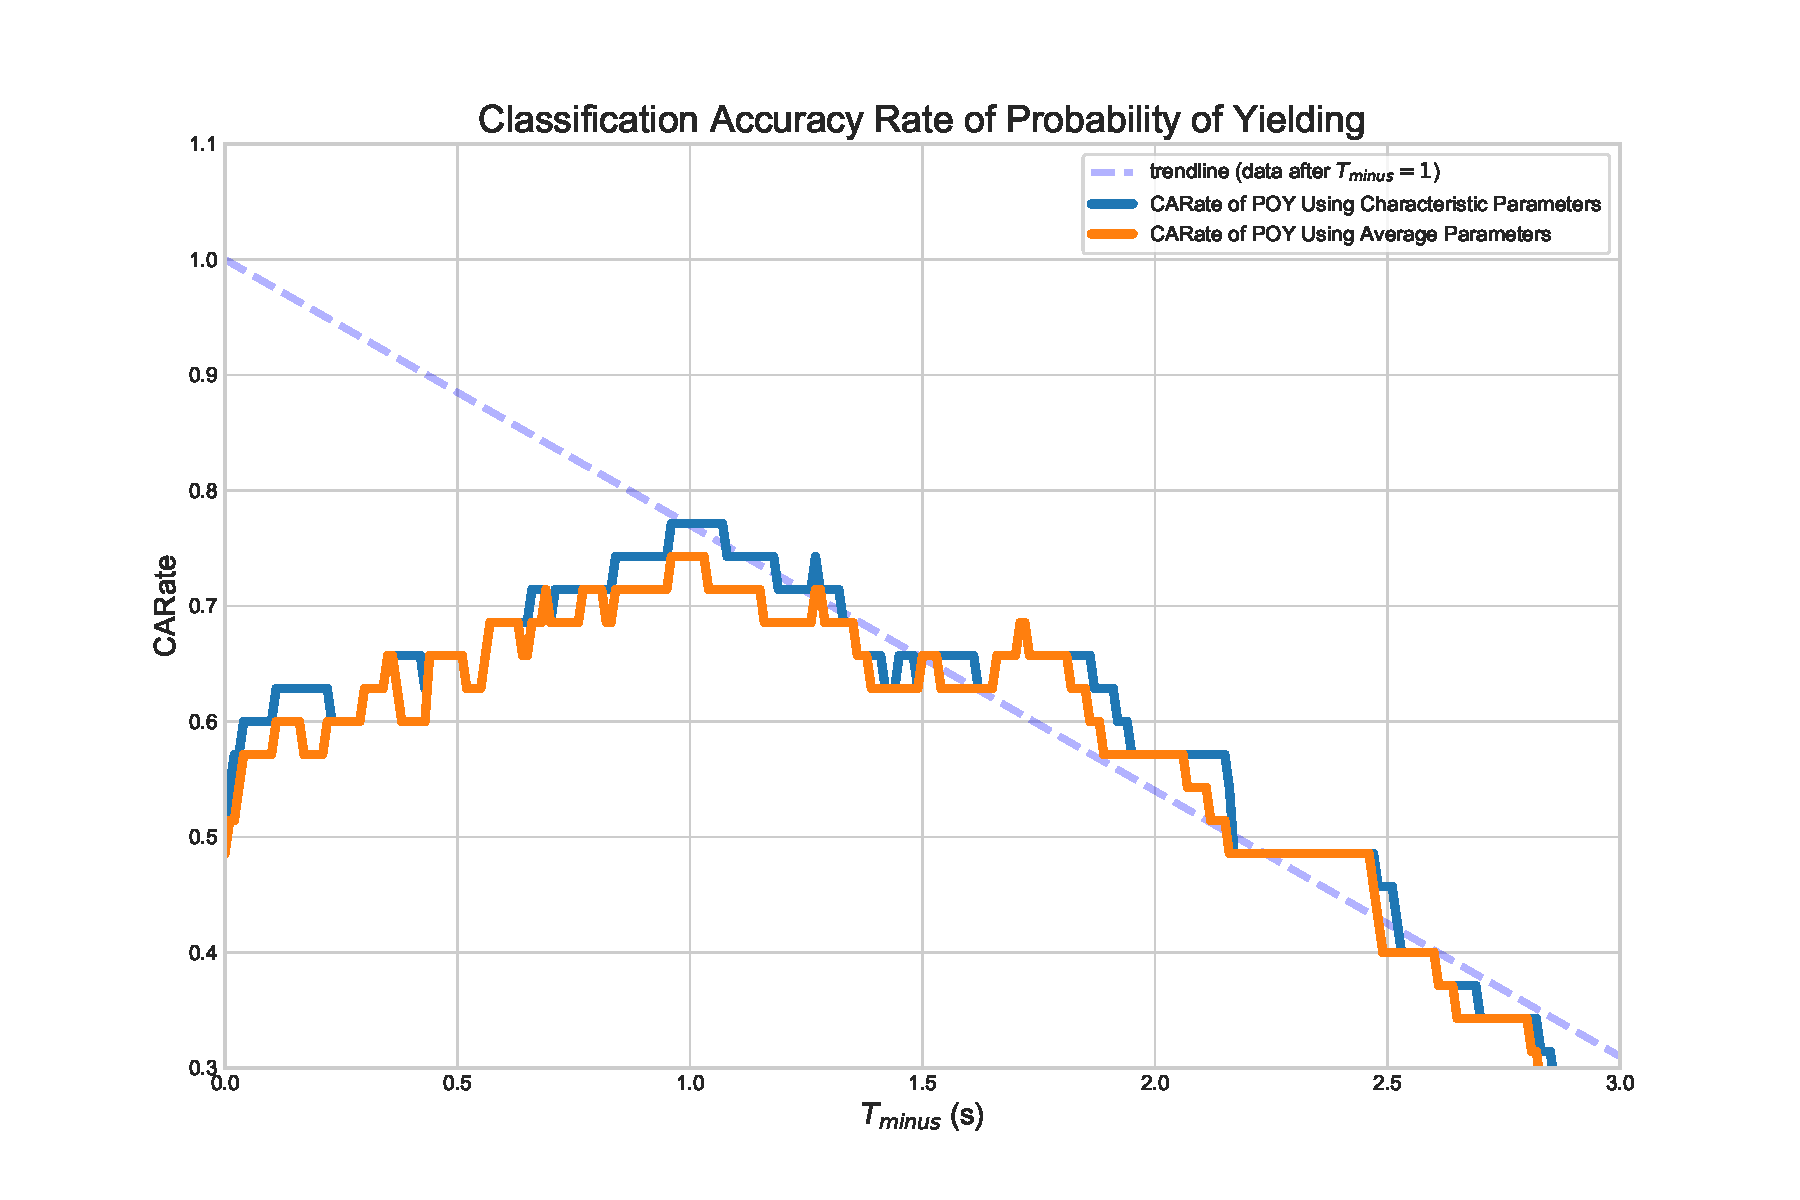
\includegraphics[width=0.7\paperwidth]{CARPOY_character_average.pdf}}
\end{center}
\caption{CARate curve of POY using average parameters and characteristic parameters are compared.}
\label{fig:CAR_comparison} 
\end{figure}


In the figure, the solid blue line indicates the CARate curve of POY using characteristic parameters (blue line for short ) while the orange line represents the CARate curve of POY using average parameters (orange line for short). The highest CARate of the blue line is around 0.78, which is higher than that of the orange line around 0.74. Despite the non-significant difference between two highest points, it is noticable that blue line is above the orange line throughout the whole $T_{minus}$ span, which gives the evidence to the supposition that the closer parameters set can give rise to larger area under the resulting CARate curve. If a more far off set of parameters are applied, e.g. the parameters set of another participant, the gaps between the resulting CARate cure of POY should be larger, owing to the more imprecise estimation for the TFA distribution. The comparison between the characteristic parameters and the parameters set of another participants are made in Fig.~\ref{fig:CAR_twoParticipants}.


\begin{figure}[htbp!]
\begin{center}
\makebox[0pt]{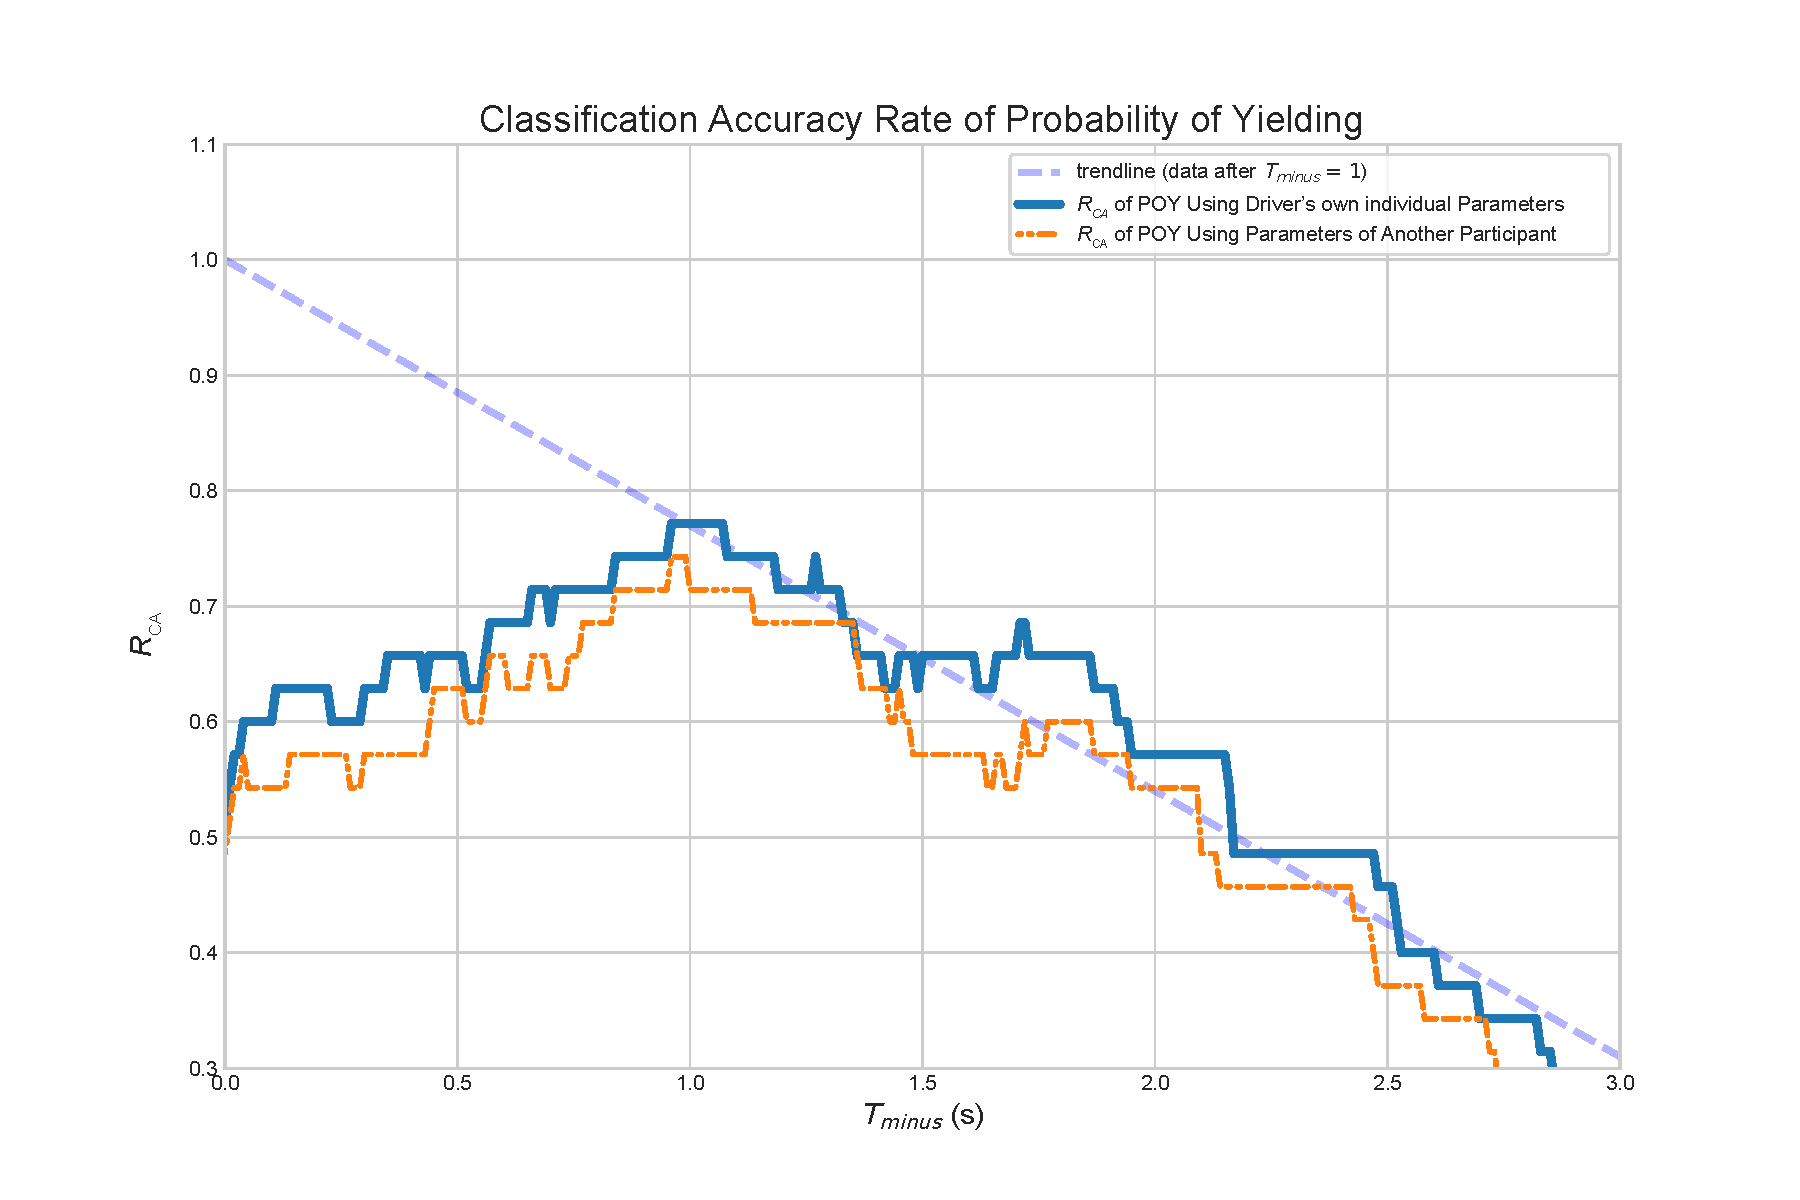
\includegraphics[width=0.7\paperwidth]{CARPOY_twoParticipants.pdf}}
\end{center}
\caption{CARate curve of POY using characteristic parameters and the parameters set of another participant are plotted.}
\label{fig:CAR_twoParticipants} 
\end{figure}

It is not hard to observe that the differences between two CARate curves are more distinct than that in Fig.~\ref{fig:CAR_comparison}, for that the values of average parameters set is closer to characteristic parameters than that of another participant.

Up to the present, the differences between the resulting CARate curves using different sets of parameter are identified. Based on this idea, creating a procedure using collected traffic data at crossroad to identify the characteristic parameters representing the driving behaviors of that area is possible. So the problem now would be, how to optimize the CARate curve so as to find the most possible parameters set representing the driver.

To solve the problem using optimization, the objective function and constraints are defined as 


    \begin{mini}|l|
	  {w}{\frac{1}{M}~\sum_{j=1}^{M}\sum_{i=1}^{N_j}{- f( { POY}_{j}(t_i, w))}}{}{}
	  \addConstraint{~2.0 \cdot {C1}_{Rmin}+{C2}_{Rmin}~}{\geq ~ 4.48}{}
	  \addConstraint{~5.2 \cdot {C1}_{Rmin}+{C2}_{Rmin}~}{\leq ~ 12.0 }{}
	  \addConstraint{~2.0 \cdot {C1}_{adec}+{C2}_{adec}~}{\geq ~ 0.01}{}
	  \addConstraint{~5.2 \cdot {C1}_{adec}+{C2}_{adec}~}{\leq ~ 3.5 }{}
	  \addConstraint{0.01~ \leq~ \gamma ~\leq ~ 0.5}{ }{}
     \label{eq:optimize_POY}
     \end{mini}

\noindent where the function ${POY}_{j}$ in the optimization problem is

\begin{equation}
    f({POY}_{j}) = 
    \begin{cases} 
      1 &~~\text{if}~~ {POY}_{j}(t, w)~\geq~0.8~\text{and yielded}~ \\
      1 &~~\text{if}~~ {POY}_{j}(t, w)~\leq~0.2~\text{and passed}~ \\
      0 &~~\text{otherwise}
    \end{cases}
\label{eq:POY_j_condition}
\end{equation}

The objective function in Eqn.~\ref{eq:optimize_POY} indicating the total area underneath the CARate curve, where the $w$ is the parameters set ($R_{min}, a_{dec}, \gamma $) maximizing the area (minimizing the negative area), i.e., bringing the parameters set into the proposed POY model could have the highest accuracy on predicting the behaviors of the driver from the experimental data. The constants $M$ and $N_j$ stand for the number of the trials in the collected data and the number of time steps in each trial with the resolution of 0.01 sec.

Due to the linearity of $R_{min}$ and $a_{dec}$, the maximum and minimum value of both parameters should occur at the maximum and minimum velocity right before braking which are 5.2 and 2.0 m/s respectively. While the definition of the $R_{min}$ is calculated from the center of one vehicle to another, the minimum distance under 2.0 m/s is also bounded by the physical model built in the simulated world, which is 4.48 meters. The maximum is then bounded by the longest between vehicles one could possibly have, which is 12 meters, the maximum distance they can see each other. As for the minimum and maximum in the constraint of $a_{dec}$, they are also restraint within the boundary set for the commend velocity sent from the joystick, which are 0.01 and 3.5 respectively.

%%%%%%%%%%%%%%%%%%%%%%%%%%%%%%%%%%%%%%%%%%%%%%%%%%%%%%%%%%%%%%%%%%%%%%%%
%%%%%%%%%%               SECTION SECTION SECTION               %%%%%%%%%
%%%%%%%%%%%%%%%%%%%%%%%%%%%%%%%%%%%%%%%%%%%%%%%%%%%%%%%%%%%%%%%%%%%%%%%%
\section{Optimization Using Simulated Annealing}
\label{sec:simAnneal}


In this research, the \ac{SA} is chosen for this optimization problem due to the non-smooth and time-consuming properties of the objective function. First published by Kirkpatrick et al. \cite{Kirkpatrick1983}, \ac{SA} is an efficient method to approximate the global optimization without using the derivative information. Despite being a global optimizer, it is not guaranteed that the solution found is an global optimum, however, the close enough variables set within limited time could be discovered.

The process of \ac{SA} is an inspiration from the annealing process in material science, where the ductility is increased during the cooling process. The key idea applied to the optimization problems is the process of the temperature dropping, which is redefined as the lowering probability of accepting a worse variables set as the solution in the optimization problem. Four essential elements in the \ac{SA} optimization problem are listed below :

\begin{itemize}

    \item \textbf{Energy function} : \\
        Usually denoted as $E_i$, representing the value of objective function using the best solution (set of variables) at the moment. In this situation, the sign of $\Delta E$ is then defining the current $move()$ to be an uphill or a downhill move.
        
    \item \textbf{Random number generator} :\\
        The function $move()$ update the solution for the optimization problem. Despite the Monte Carlo method is applied, a well defined update procedure can solve the optimization problem with efficiency.
        
    \item \textbf{Worse case accepting probability} :\\ 
        Defining the probability $P_i$ that whether to accept a worse solution is the essential element for the \ac{SA} to jump out of the local minimum. It is usually in the form of
        
        \begin{equation}
             P_i = \exp{\frac{- \Delta E}{T_i}}
        \label{eq:SA_tempDrop}
        \end{equation}
    
        where the $\Delta E$ represents the difference between the objective function value generated by the new solution and the best one so far. When a worse solution is generated, the value $P_i$ is compared to a random number, and the worse solution is accepted if $P_i$ is greater than the random number. Hence, larger the $\Delta E$ values will reduce the chance a worse solution being accepted. On the contrary, higher the current temperature indicating a higher chance of adopting the worse solution.
    
    \item \textbf{Annealing ( cooling ) schedule} : \\
        Within the \ac{SA}, the temperature drop is governed by equation

        \begin{equation}
             T_{i+1} = T_{i} \cdot \exp{\frac{T_{factor, i} \cdot i}{N}}
        \label{eq:SA_tempDrop}
        \end{equation}

        where the $T_{factor}$ is defined as

        \begin{equation}
            T_{factor, i} = - \ln{\frac{T_{i}}{T_{min}}}
        \label{eq:SA_tFactor}
        \end{equation}

        The temperature decay is based on the Newton's law of cooling with little modification to end the optimization process within designated number of steps $N$. In the equation, the $T_i$ is the current temperature and $T_min$ is the target temperature of cooling ( i.e. the environment temperature in the annealing process ). 
\end{itemize}

In our case, the energy function $E_i$ is defined by the objective function in Eqn.~\ref{eq:optimize_POY}, where the $\Delta E$ is found in every iteration by calculating $(E_{i+1} - E_i)$ after the new set of variables are generated by function $move()$ and examined to satisfy the constraints. If a better solution is found ( meaning that $\Delta E < 0$ ), the best solution is replaced with the new one. Otherwise, the probability $P_i$ is then compared to a random number to decide whether to accept the worse solution. The process then iterate $N$ times (until the temperature drops to the environment temperature), or one of the termination conditions is reached. 

The results of the optimization are shown in Table ~\ref{table:SAresults}, and the parameters used for the \ac{SA} in the optimization problem are listed in Table ~\ref{table:SAparams}.


\begin{table}[htbp]
\caption{Table for results of the proposed optimization problem.}
\begin{center}
\label{table:SAresults}
\begin{tabular}{l l c c c c c c}
& & \\ % put some space after the caption
\hline
\textbf{Optimization Number} &  &\textbf{${C1}_{Rmin}$} &\textbf{${C2}_{Rmin}$} &\textbf{${C1}_{adec}$} &\textbf{${C2}_{adec}$} & \textbf{$\gamma$} & \textbf{Area}\\
\hline
1st Optimization  &  & 0.362 & 7.91 & 0.0460 & 0.954 & 0.460 & -205.40 \\
2nd Optimization  &  & 0.401 & 7.86 & 0.224 & 0.563 & 0.443 & -205.37 \\
3rd Optimization  &  & 0.322 & 7.91 & 0.106 & 0.941 & 0.434 & -205.23 \\
4th Optimization  &  & 0.456 & 7.49 & 0.102 & 0.824 & 0.444 & -205.37 \\
5th Optimization  &  & 0.346 & 7.95 & 0.145 & 0.812 & 0.448 & -205.37 \\
\textbf{Characteristic}  &  & \textbf{0.166} & \textbf{6.19} & \textbf{0.465} & \textbf{0.377} & \textbf{0.114} & \textbf{-183.89} \\
\hline
\end{tabular}
\end{center}
\end{table}

\begin{table}[htbp]
\caption{Table for parameters used in the Simulated Annealing.}
\begin{center}
\label{table:SAparams}
\begin{tabular}{l l c c c}
& & \\ % put some space after the caption
\hline
\textbf{Parameters} &   & Values \\
\hline
Start Temperature    &  120  \\
End Temperature      &  0.02 \\
Steps                & 100000 \\

\hline
\end{tabular}
\end{center}
\end{table}

\begin{figure}[htbp!]
\begin{center}
\makebox[0pt]{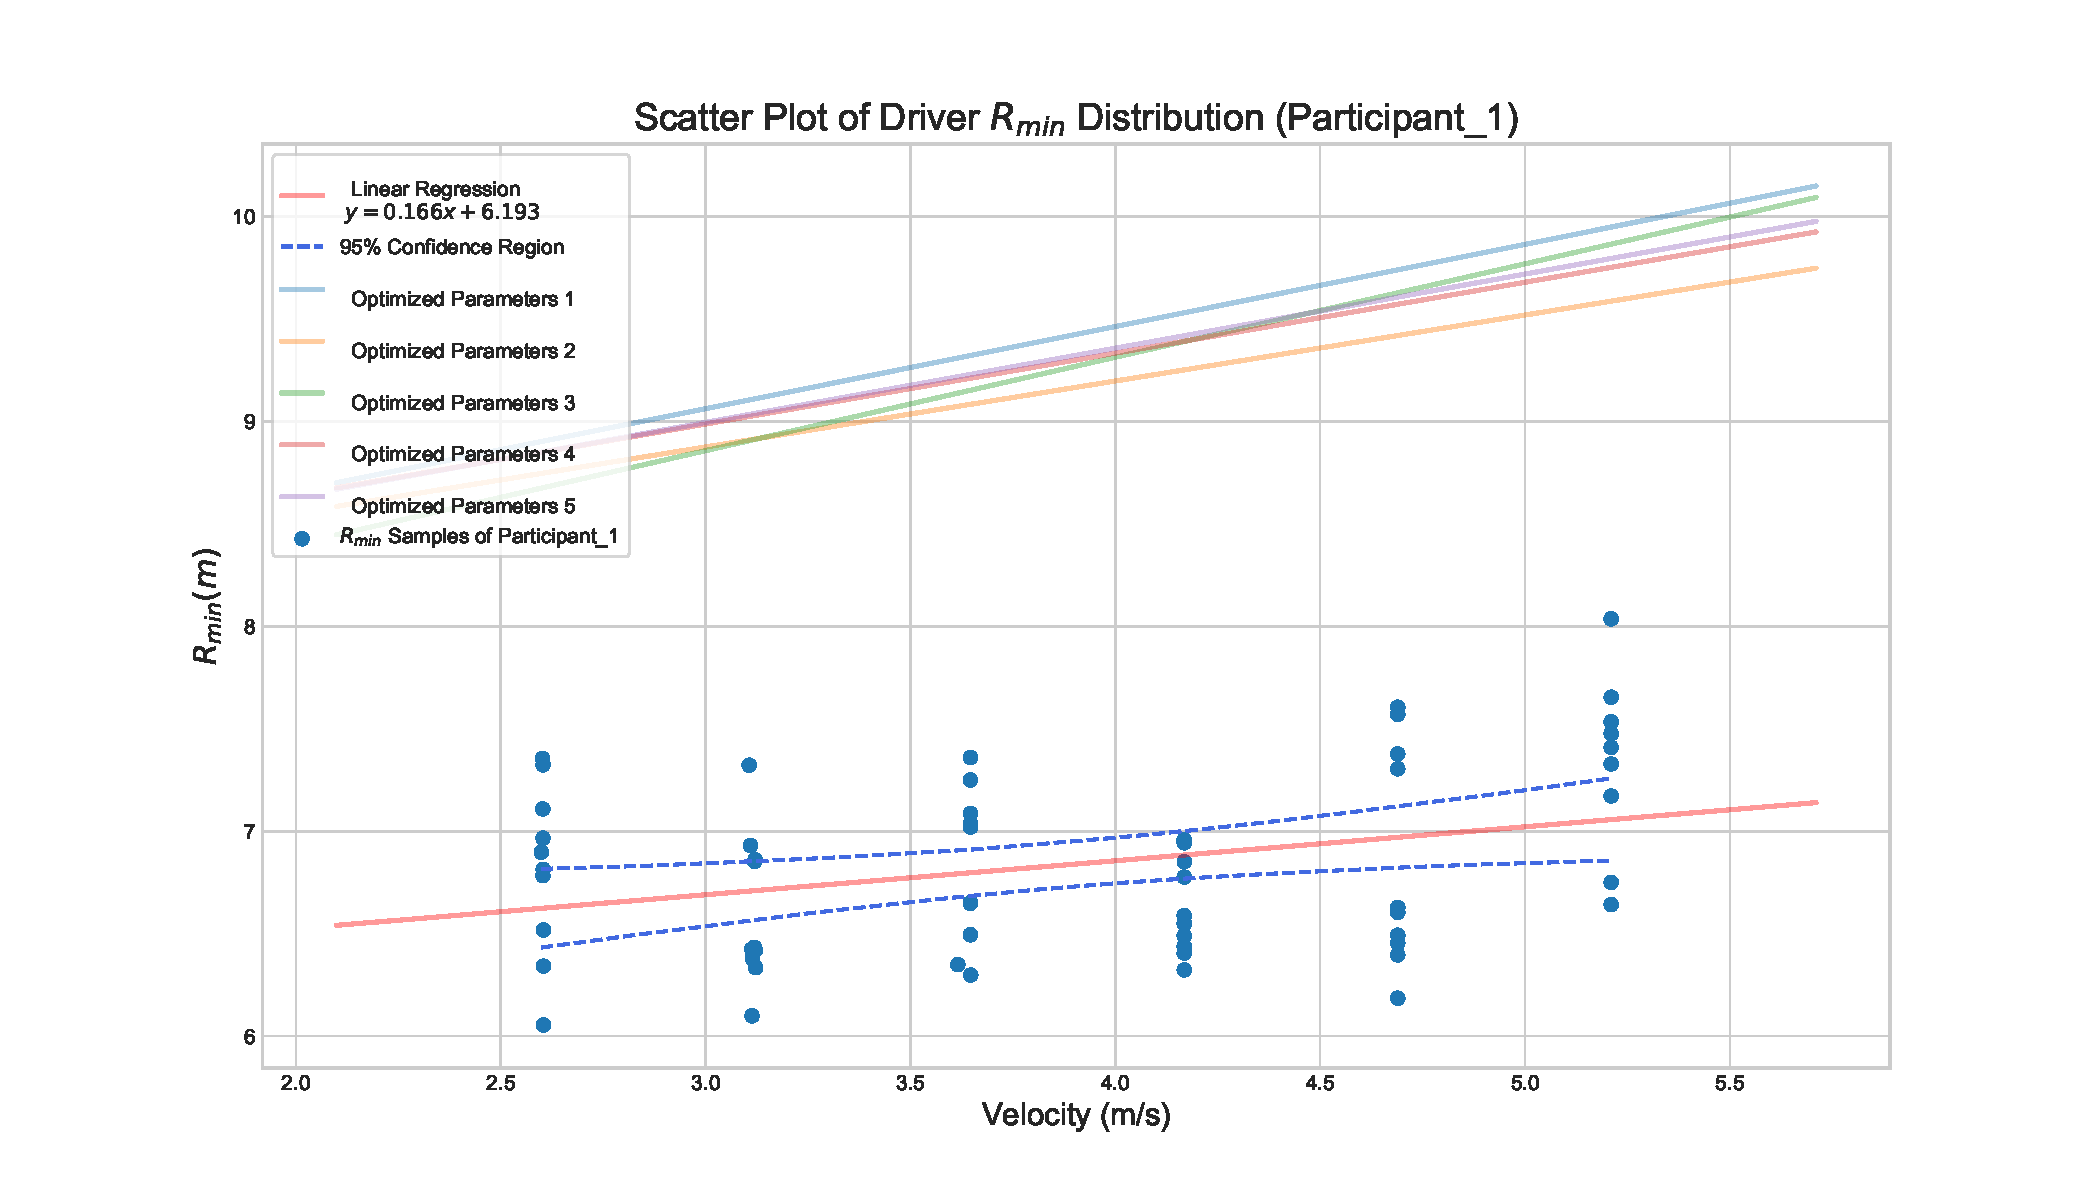
\includegraphics[width=0.7\paperwidth]{Participant_1_R_MIN_optimized.pdf}}
\end{center}
\caption{Optimized parameters of $R_{min}$ are compared with characteristic parameters.}
\label{fig:RMINParamOptimChara} 
\end{figure}

\begin{figure}[htbp!]
\begin{center}
\makebox[0pt]{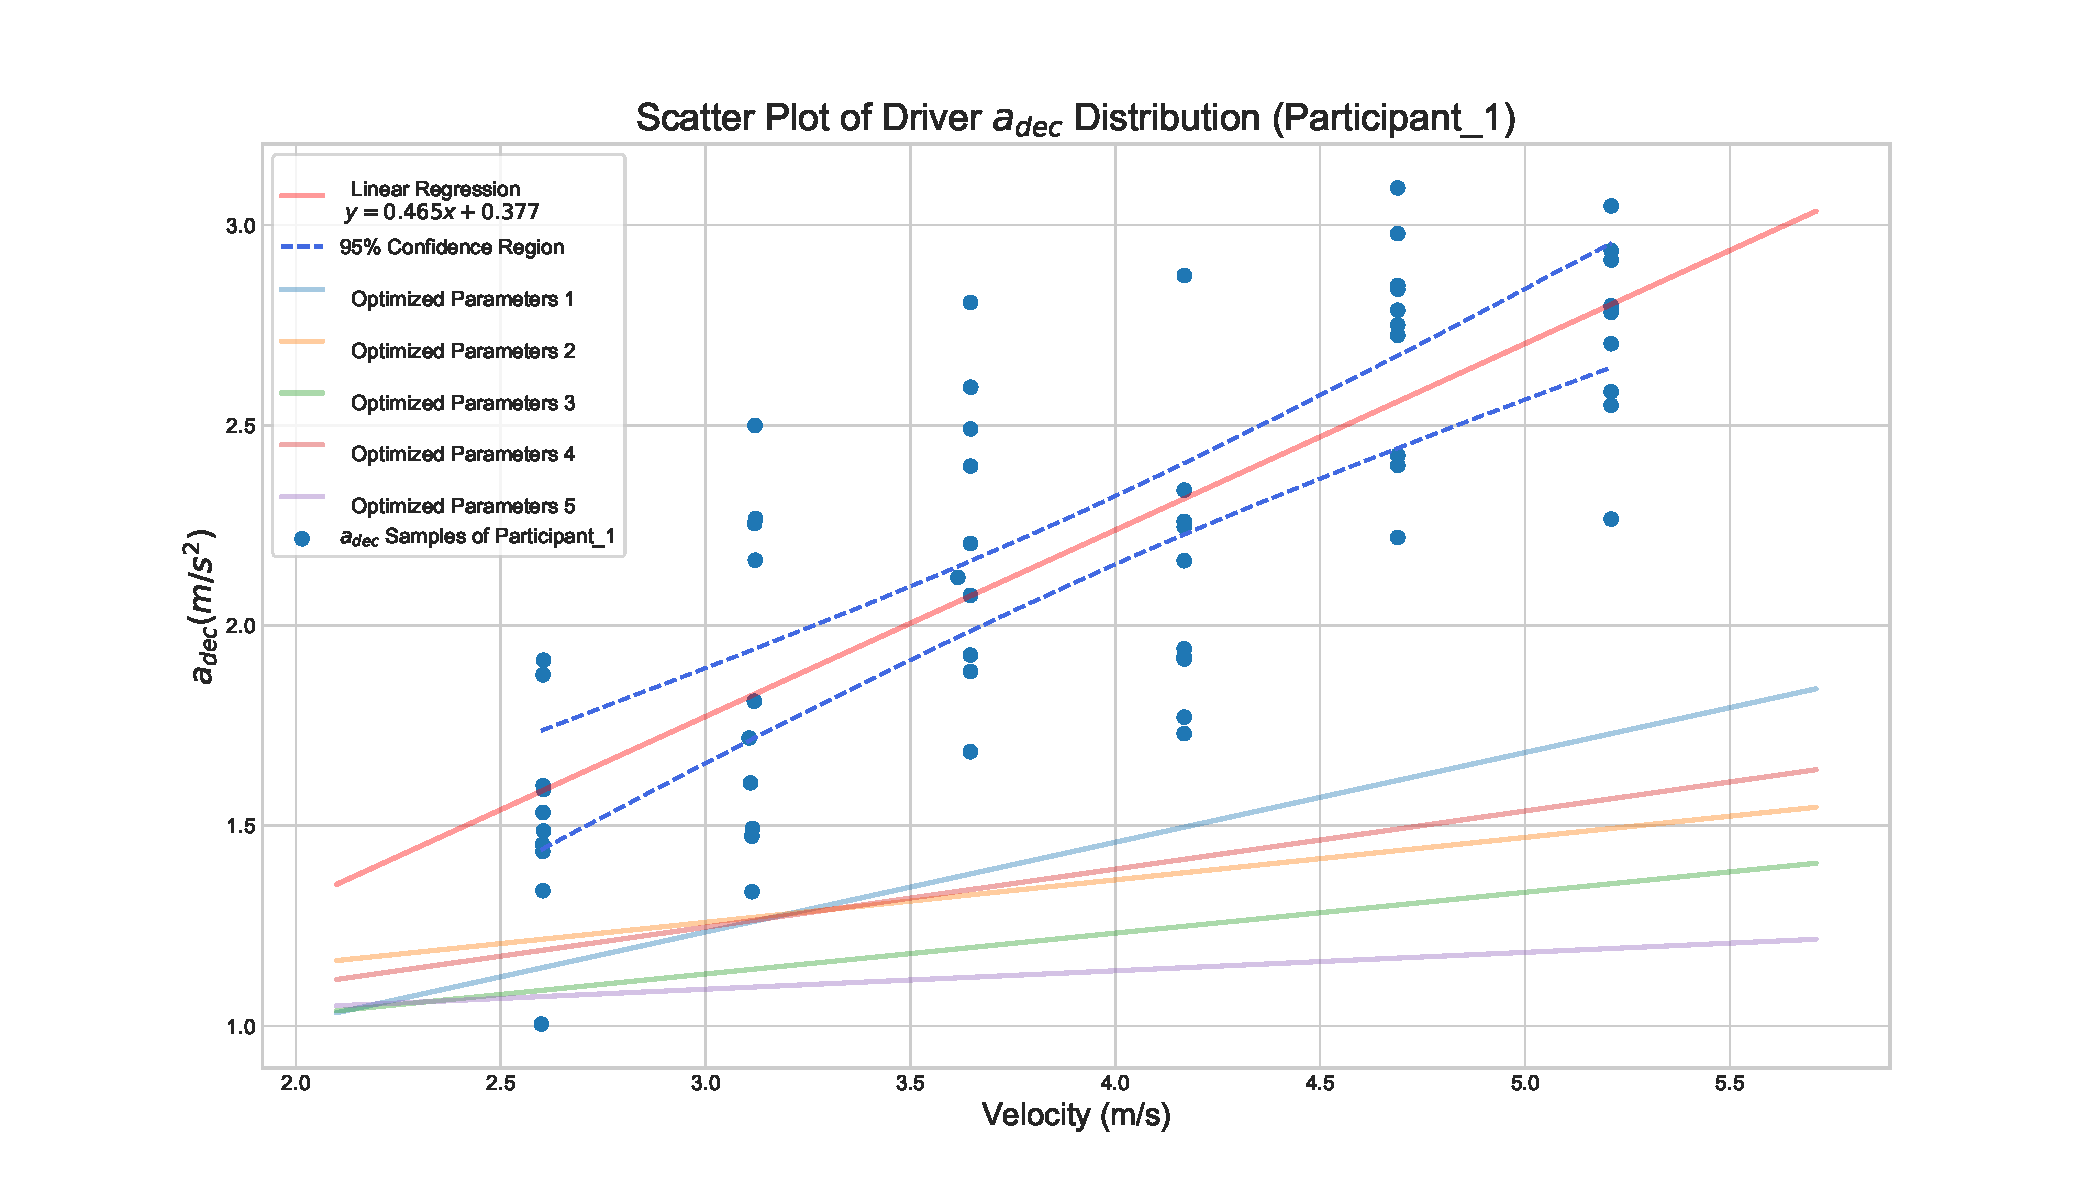
\includegraphics[width=0.7\paperwidth]{Participant_1_A_DEC_optimized.pdf}}
\end{center}
\caption{Optimized parameters of $a_{dec}$ are compared with characteristic parameters.}
\label{fig:ADECParamOptimChara} 
\end{figure}

The optimized parameters for $R_{min}$ and $a_{dec}$ are shown in Fig.~\ref{fig:RMINParamOptimChara} and Fig.~\ref{fig:ADECParamOptimChara}.While in Fig.~\ref{fig:CAR_optimParam}, the CARate curves using optimized parameters listed in Table ~\ref{table:SAresults} are plotted together with the CARate curves using characteristic parameters. In Fig.~\ref{fig:RMINParamOptimChara} and Fig.~\ref{fig:ADECParamOptimChara}, the corresponding lines representing the linear equation using ${C1}$ and $C2$ as the coefficient and constant are forming a cluster in plots of $R_{min}$. While in $a_{dec}$, the lines are not as ordered at higher velocities. 


However, when looking into Fig.~\ref{fig:CAR_optimParam}, all of the optimized CARate curves are overlapped and the area under the curves are larger than the characteristic parameters. Some might wonder, does this implied that the optimized parameters are a better set of parameters that can explain the behavior of the driver? To answer this question, first, the POY curves using the optimized parameters should be examined.

\begin{figure}[htbp!]
\begin{center}
\makebox[0pt]{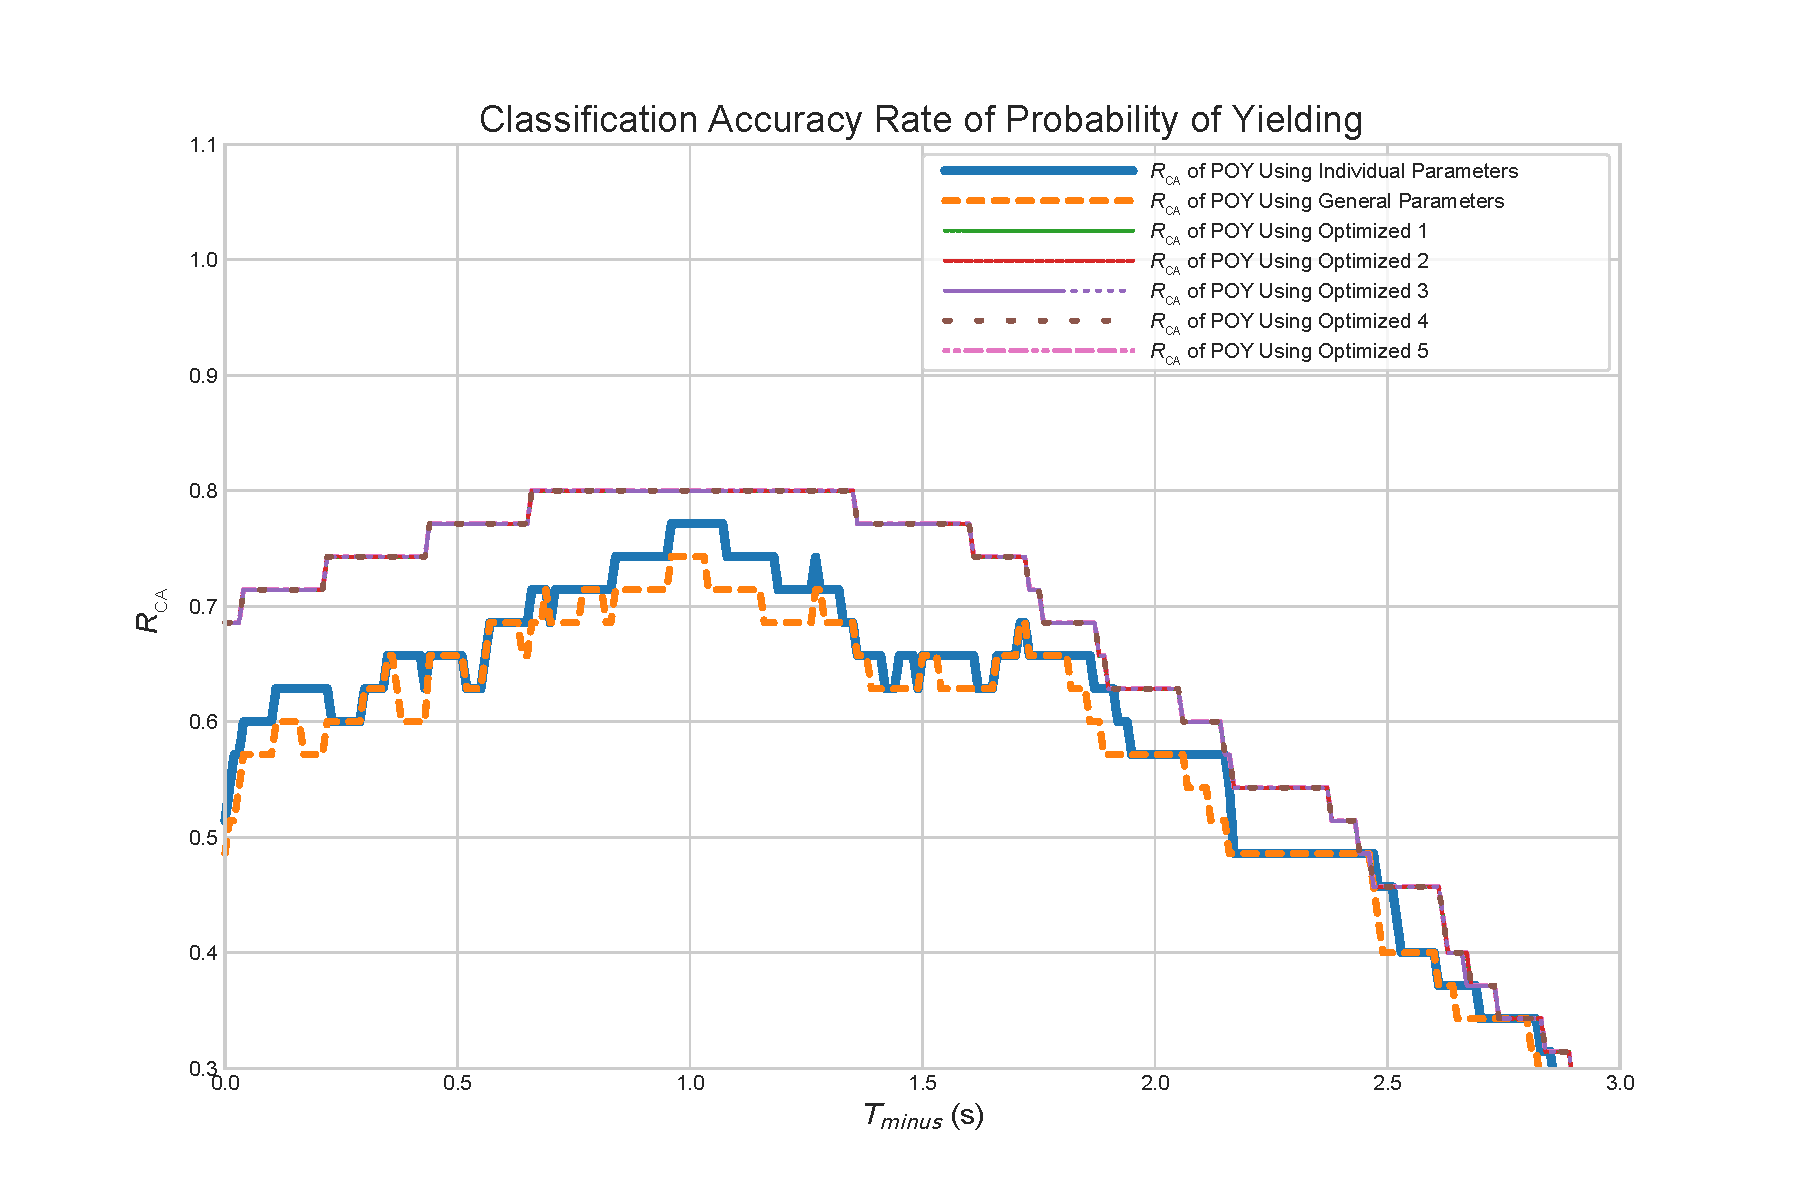
\includegraphics[width=0.7\paperwidth]{CARPOY_optimizedParam.pdf}}
\end{center}
\caption{CARate curve of POY using characteristic parameters and optimized parameters are plotted.}
\label{fig:CAR_optimParam} 
\end{figure}

As shown in Fig.~\ref{fig:trial003OptimChara} and Fig.~\ref{fig:trial077OptimChara}, the POY curves of the optimized parameter (here the parameters set Optimized 1 is chosen ) rose way earlier than using the characteristic parameters. This implies that the the POY with optimized parameters is very sensitive to all the accelerations, so at the instance the vehicle begins to decelerate, the action is considered as having the intention to yield. Yet, being too sensitive to accelerations will result in the bumpy curves, making the meaning of POY curves not understandable, and will sometimes generate false results. For example, the rises of POY curves using optimized curves in both figures are way early than the interactions begin, which happen around the distance to the node is about 15 meters. The optimized parameters do have a better CARate curve, but this does not suggest a more accurate prediction. Some modifications for the objective function are required, so the characteristic parameters could be identified more accurately.


\begin{figure}[htbp!]
\begin{center}
\makebox[0pt]{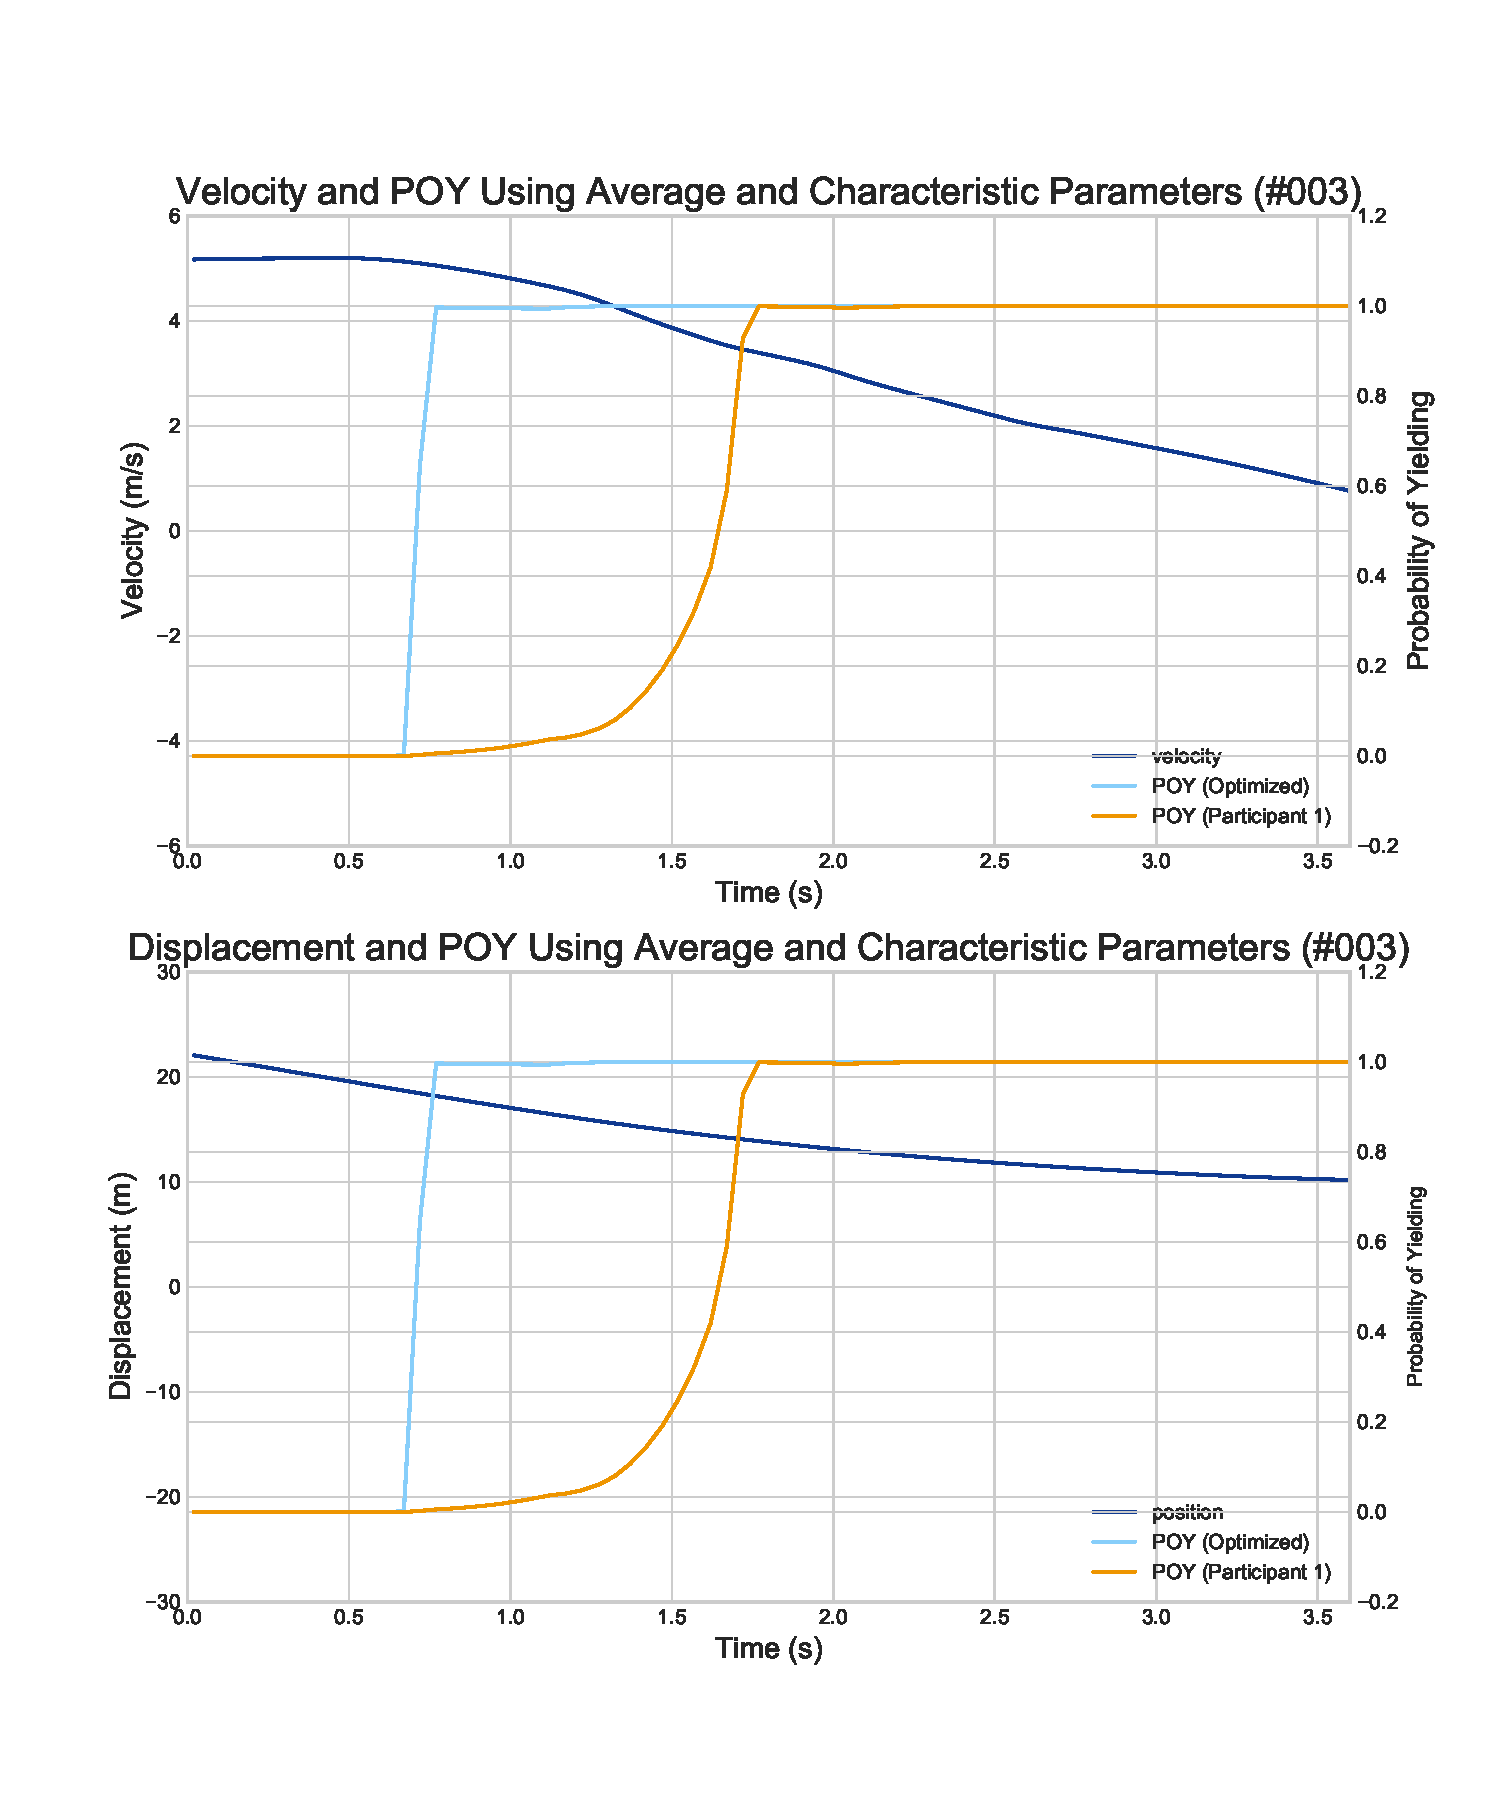
\includegraphics[width=0.7\paperwidth]{optimized_trial_003.pdf}}
\end{center}
\caption{Trial \#003 using the optimized parameters and the characteristic parameters.}
\label{fig:trial003OptimChara} 
\end{figure}

\begin{figure}[htbp!]
\begin{center}
\makebox[0pt]{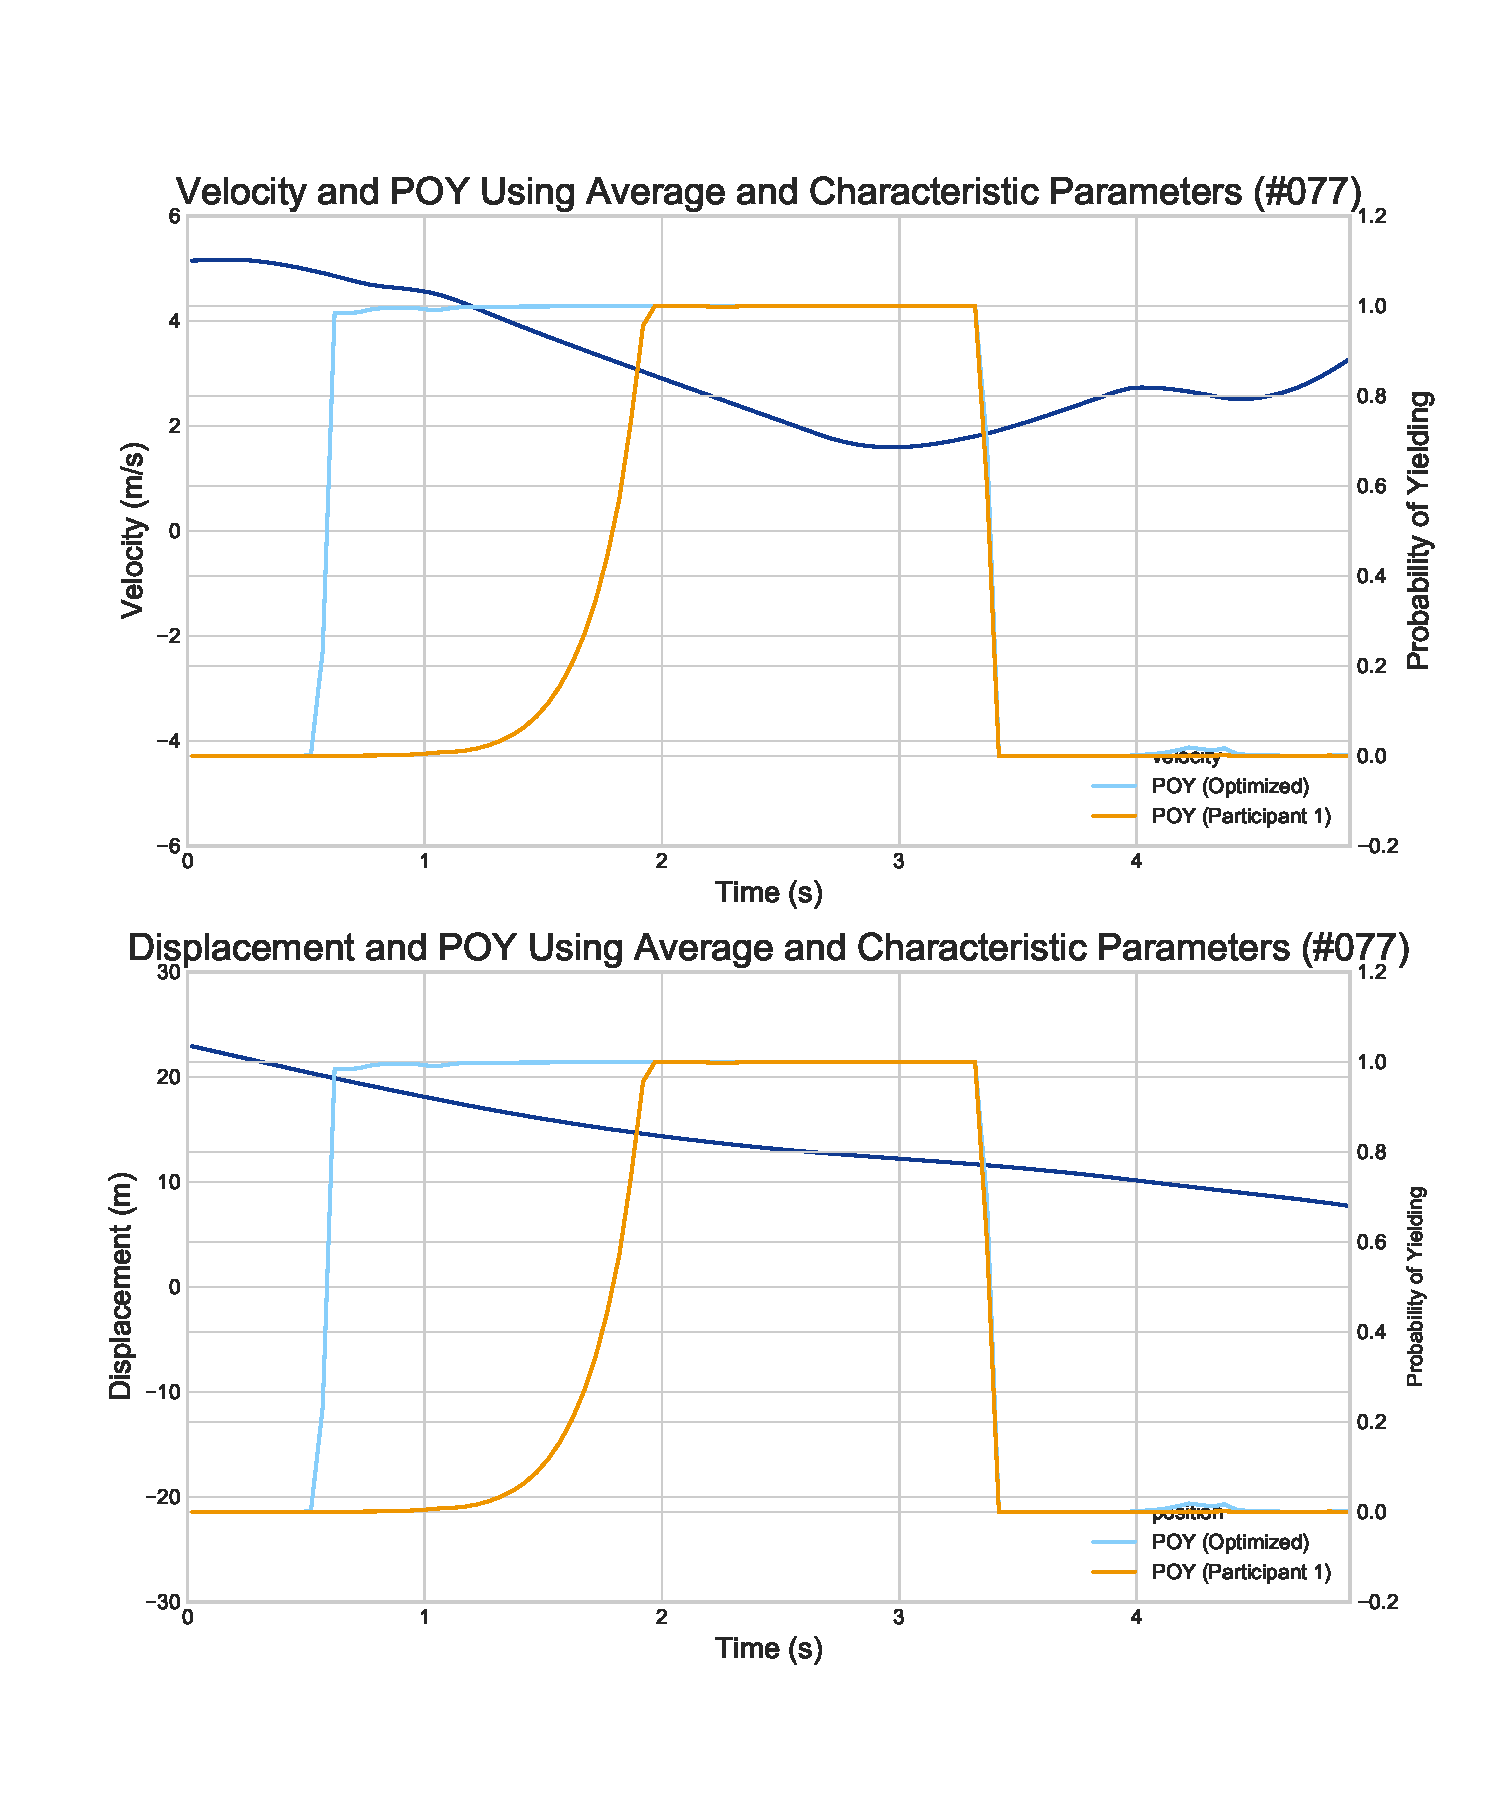
\includegraphics[width=0.7\paperwidth]{optimized_trial_077.pdf}}
\end{center}
\caption{Trial \#077 using the optimized parameters and the characteristic parameters.}
\label{fig:trial077OptimChara} 
\end{figure}


In this chapter, a characteristic parameters identification procedure was developed. From the examinations of the POY curves using the characteristic parameters of the driver and the average parameters, the idea of using the results of POY curves and CARate curves to identify the characteristic parameters was generated. After proving it using the CARate curve, an optimization problem was constructed with the area under the CARate curve as the objective function. Despite some improvements are needed to have a more precisely parameters identification, this procedure provides a preliminary method for characteristic parameters recognition.